\documentclass[12pt,titlepage]{articles}
\usepackage[ngerman]{babel}
\usepackage[utf8]{inputenc}
\usepackage{color}
\usepackage[a4paper,lmargin={4cm},rmargin={2cm},
tmargin={2.5cm},bmargin = {2.5cm}]{geometry}
\usepackage{amssymb}
\usepackage{amsthm}
\usepackage{graphicx}
% Makros für allgemein nützliche Dinge wie Korrekturfeedback :-)
% Dies hier auskommentieren, falls du in der Ansicht keine Kommentare sehen willst. 
%\newcommand{\dwi}[1]{}
% Dies hier mit % kommentieren, falls du in der Ansicht keine Kommentare sehen willst. 
\newcommand{\dwi}[1]{\textcolor{red}{\footnotesize#1}}
%\newcommand{\dwi}[1]{\textcolor{red}{\footnotesize}}

% Tests..
%\newcommand{\dwi}[1]{\marginpar{\textcolor{red}{\tiny#1}}}

\begin{document}
\title{DevOps meets OSS: Automatisierte Integration von OSS in die DevOps-Produktentwicklung\\}
\author{Claudia Arnold}

\maketitle

\begin{abstract}
   Unter dem Begriff OSS bekannt, bietet die Open Source Software eine Reihe an Möglichkeiten im Bereich der Softwareentwicklung. Durch die sinkenden Nutzungesbescchränkungen im Vergleich zur konventioneller Software gilt OSS als ein Instrument zur schnellen Integration von Software in die eigene Entwicklung.  
   \dwi{hier kommt noch mehr oder? könnte sich lohnen dies mal im gesamtscope der arbeit zu formulieren um sich den rahmen bewusst zu machen.}
\end{abstract}

\newpage  
\begin{center} 
    \vspace*{\fill}
    \textit{‘Free software’ is a matter of liberty, not price. To understand the concept, you should think of ‘free’ as in ‘free speech,’ not as in ‘free beer’.}
    \newline
    \newline - Richard Matthew Stallman
    \vspace*{\fill}
\end{center}

\newpage
\dwi{also es ist der knaller was du hier an wissen angehäuft hast, respekt. da hast du eine ordentliche recherche gemacht.
die aufgabe ist allerdings jetzt, das wissen auf ein transportierbares maß zu reduzieren und zu fokussieren
- hier gilt qualität vor quantität, und das ist auch ein wesentlicher teil deiner leistung. nicht alles was du 
zum thema weißt muss notwendigerweise als text in deine arbeit, hier und da liest es sich als ob du in einem paper ein
für dich wertvolles konzept gefunden hast du dann einen satz dazu irgendwo einfügst wo er am besten passt.
hier sind gezielte referenzen und knackige sätze noch viel wertvoller. du weißt .. es muss immer einer arbeiten, der autor oder der leser.
und je weniger der leser arbeiten muss desto besser ist deine arbeit. du schreibst ja auch (noch?) keine doktorarbeit :-)}
\section{Einleitung}
\begin{quote}
\textit{In real open source, you have the right to control your own destiny}\newline -Linus Torvalds
\end{quote}

Verändertes Konsumentenverhalten, schnelle Reaktion auf veränderte Kundenwuensche und Time-to-Market sind wesentliche Anforderungen, die für den wirtschaftlichen Erfolg eines Unternehmens insbesondere in Zeiten der Digitalisierung kennzeichnet sind und daher große Herausforderungen mit sich bringen. git staDie daraus resultierenden steigenden Anforderungen an neuer Funktionalität und die damit verbundene stetige Weiterentwicklung erfordern in erster Linie eine neue Dynamik innerhalb der Entwicklug, Konzepte und Tools. In diesem Zusammenhang wird der Softwareentwicklungsprozess nach agilen Methoden unablässig und gehört in den meisten Unternehmen bereits zum Standard einer IT-Organisation. 

In diesem Rahmen kommt der Ansatz des DevOps zum Tragen, nach dessen Grundsätzen der Softwareentwicklungsprozess, angefangen von der Idee, über die schnelle Entwicklung bishin zum Einsatz innerhalb der Produktivumgebung, durchgeführt wird. DevOps ist ein Kofferwort aus den Begriffen Development und IT-Operations und beschreibt im Wesentlichen die technische und organisatorische Verbindung zwischen der Softwareentwicklung und der Systemadministration. Charakterisch sind verkürzte Releasezyklen in einem inkrementellen Prozess und ein hoher Automatisierungsgrad, wodurch eine exakte Planung, Vermeidung von kritischen Fehlern und eine schnelle Reaktion auf Kundenanforderungen ermöglicht wird. Wesentliches Ziel von DevOps ist es, die gesamte Entwicklung transparent, flexibel und agil zu gestalten, wodurch die Produktivität und Effizenz maßgeblich gesteigert und das endgültige Produkt schneller zum Kunden ausgeliefert werden kann. 

Neben der agilen Softwareentwicklung ist ein weiteres wesentliches Kennzeichen des DevOps-Konzeptes die Grundsätze des Lean Manufactoring, nach denen die Minimierung von Verschwendung und die Maximierung der Produktivität im Vordergrund steht. Dabei spielt insbesondere die Wiederverwendung von Software eine wesentliche Rolle. Anstatt einer zeit- und kostenintensiven Neuentwicklung von Software, bleiben viele allgemeine oder wiederholende Funktionalitäten innerhalb eines neuen Projektes oftmals gleich und müssen demnach nicht verändert werden. Vor diesem Hintergrund sparen Entwickler viel Zeit und Ressourcen, indem Quellcode, Templates oder Algorithmen wiederverwendet werden, was wiederrum dem Grundgedanken von DevOps entspricht. 

Ausgehend hiervon ist die Integration von bestehenden Softwarekonzepten ein wesentlicher Vorteil, wodurch die Verwendung von Open Source Software zunehmend an Bedeutung im Unternehmensfeld gewinnt. Als eine realistische Alternative zu herkömlicher Software, erlangte die Open-Source-Bewegung mit der Idee von frei zugänglicher Software in den letzten Jahrzehnten immer mehr an Popularität. Unter Open Source Software versteht man einen öffentlich zugänglichen Quellcode, den jeder einsehen, verändern und für sich nutzen kann. Im Gegensatz zur herkömlicher proprietärer Software, erhalten Nutzer eine Open Source Software meist kostenlos und ohne weitere Kosten für Lizenzvereinbarungen. Durch den unmittelbaren Zugang zum Quellcode, haben Entwickler die Möglichkeit einerseits, am Quellcode mit nur wenigen Ressourcen zu experimentieren und zu überprüfen, ob sich dieser ein wiederkehrendes Problem innerhalb des Projektes beinhaltet oder anderseits nach der jeweligen Problematik zu individualisieren und zu verändern. Die Notwendigkeit einer kosten- und zeitspielige Entwicklung entfällt und die Verwendung von bereits gelösten Paradigmen rückt in den Vordergrund.   

% Häufige Vorgehensweise: Moduale Architektur von Open-Sorce projekten
% Beispiele an OSS aufzeigen: Betriebssysteme, Server-Anwendungen oder Office-Produkte
% Evtl hier nochmal auf Linux, als erstes populäres Produkt im OSS-Bereich eingehen 

Das daraus resultierende Innovationspotenzial kann, basierend auf der freien Gestaltungsfreiheit die OSS im Gegensatz zur kommentieller Lizenzsoftware ermöglicht, genutzt werden, Ideen umzusetzen ohne zu stark an unternehmensinterne Vorgaben gebunden zu sein oder unternehmensinterne Prozesse oder Prozessabläufe in die Entwicklung einzubinden. Vor diesem Hintergrund kann eine umfassende Integration von Open Source Software in vorhandene Unternehmenstrukturen im Bereich der Entwicklung, ausschließlich in einem agilen Umfeld durchgeführt werden, womit DevOps als ideale Plattform geeignet ist.  

Trotz der Freiheiten, die Open Source Software offensichtlich bietet, unterliegen die meisten Projekte rechtlichen Schutzmaßnahmen, einschließlich dem Marken- Patent- und Urheberrecht. Aufgrund dessen können, aus der Verwendung von OSS resultierende Lizenzfragen oder rechtliche Konsequenzen, zu einer maßgeblichen Einschränkung insbesondere im Hinblick auf eine mögliche Verteilung oder Weitergabe an Dritte führen, die von Unternehmen genau analysiert und überprüft werden muss.  

In dieser Thesis werden die grundsätzlichen Vorteile und Risiken, die sich aus den verschiedenen Lizenzvereinbarungen bei der Verwendung von OSS ergeben analysiert und die Migration in den Devops-Emntwicklungsprozeess dargestellt. Verdeutlicht wird die Themenstellung anhand der ausgeführten Analysen anahnd eines Beispiels bei der msg Systems. 




Durch die freie Verfügbarkeit des Quellcodes, die entfallenen Lizenzkosten für den Einsatz und die freie Weiterentwicklungsmöglichkeiten, erweist sich OSS als eine einfache und kostengünstige Innovationsquelle für Unternehmen. 

Dabei reicht das Anwendungsfeld für die Verwendung von OSS in diesem Zusammenhang von der Automobilindustrie bis zur Versicherungsbranche und steht daher im direkten Wettbewerb zu proprietären Softwareangeboten. 

\subsection{Problemstellung}
Wie bereits beschrieben unterliegen 





In diesem Abschnitt wird beschrieben, welche derzeitige Problemstellung innerhalb der DevOps Produktentwicklung bei der Integration von FOSS vorliegt, die mittels der Thesis gelöst bzw verbessert werden kann. Insbesondere wird dabei auf die derzeitige Ist-Situation eingegangen, welche Herausforderungen momentan vorliegen (bei msg und allgemein) und wie der aktuelle Stand der Wissenschaft in diesem Kontext ist. 
Zudem wird eine Herleitung zu den Ziel und den Forschungsfragen dieser Thesis hergestellt.  

\subsection{Ziel und Fragestellung}
Unter diesen Gesichtspunkten lassen sich fünf Forschungsfragen für diese Arbeit wie folgt ableiten:\\ 

1. Welche praxisrelevanten Informationen können aus OSS extrahiert und verwendet werden?\\ 

%(Lizenzmodelle)
% was soll die Zielgruppe dieser Frage sein? --> Mehrheitlich die Devops-Umgebung (dh. Entwickler, Softwaredienstleister)
% zunächst grundlegende Informationen aufzuzeigen, danach den praxisrelevanten Kontext beachten (Überblick schaffen)


2. Welche Einschränkungen sind bei der Verwendung von OSS in Hinblick auf die verschiedenen Lizenzinformationen zu berücksichtigen?\\ 

%(Haftungs-/Garantiebedingungen, Autorenhinweise, Copyleft-Bedinungen)
%Anhand von praxisrelevaten Lizemzmodellen, werden ausschließlich diese mit Einschränkungen versehen, die anderen eher erwähnen. 
%Praxisrelevanz wird anhand des beschriebenen Produktes bei msg festgelegt


3. Welche prozessualen Anpassungen müssen anhand der gewonnenen Erkenntnisse getroffen werden, um auf mögliche Veränderungen in den Lizenzinformationen reaktionsschnell vorbereitet zu sein?\\ 

% GEnerell HAF-Projekt verwenden, kein exaktes Produkt da der Entwicklungspriozess gleich abläuft. 
% Ist-zustand muss exakt dargestellt werden, (Manuelle Aktualsierung aller FOSS-BEdinugngen und Deklarationen erforderlich) + gängiger Prozess muss designt werden!
% Ist-Zustand: OSS wird genommen und modifiziert und im Rahmen der Unternehmung ausgeliefert 
% --> Daraus ergibt sich der Soll- Zustand, indem die Einschränkungen basierend auf Frage 2, zum Tragen kommen und die Situationen aufzeigen, in dem sich der Ist-Zustand verändern muss --> Veränderungen am Prozessmodell angepasst 
% Welche Stakeholder sind beteiligt, wer hat welche Verantwortung/Pflichten/Aufgaben --> welche Informationen müssen weitergegeben werden
%Hieraus ergeben sich je nach beteiligten Stakeholder, unterschiedliche Verantwortungen, Pflichten und Aufgabengebiete.





%% (evtl.) Proof of Concept
%Prozess wird dargestellt --> Wie wird dieser durchgeführt/Wie wird erreicht?


4. Wie können relevante Lizenzinformationen und haftungsbedingte Anforderungen anhand eines Produktes automatisiert aus den verwendeten Lizenzmodellen aus OSS herausgearbeitet werden?\\ 

%(Programm, Makros ???)\\
%Soll-Prozess wird implentiert --> Konkrektes Beispiel
%Automasierungsgrad muss hoch sein, in Sinne von Devops


5. Wie kann die Transparenz der gesammelten Informationen insgesamt sichergestellt werden?\\ 

%(Wie kommen die Informationen schnell an das Devops-Team)\\ 
%Transparenz/Kommunikation muss gewährleistet werden --> Änderungen des Lizenzkonstellation muss tranzparent gestaltet werden (zb. Dashboards, Alters, REports)
%Dokumentation  

Ziel dieser Arbeit ist es, zunächst Informationen im Bereich DevOps und OSS zu gewinnen und dabei insbesondere die Einschränkungen der unterschiedlichen Lizenzmodelle zu beschreiben. Hierzu wird insbesondere auf die juristischen Regelungen der OS-Linzenzen und die rechtlichen Konsequenzen bei einem Nichteinhalten der gesetzlichen Schutzmaßnahmen, die sich für ein Unternehmen ergeben kann, näher eingegangen. In diesem Zuge werden prozessuale Anpassungen im DevOps-Prozess vorgenommen, die sich einerseits durch die Auslieferung des Softwareproduktes nach der Modifikation von OSS oder anderseits durch Änderungen von Lizenzbestimmungen während des Softwareentwicklungsprozesses ergeben. Ausgehend von den prozessualen Veränderung soll innerhalb der praxisorientierten Umsetzung, eine Möglichkeit dargestellt werden, wie die gewonnenen Ergebnisse automatisiert herausgearbeitet werden und der Informationsfluss innerhalb des ganzen DevOps-Teams sichergestellt werden kann.
 

\subsection{Aufbau dieser Arbeit}
Der Aufbau dieser Arbeit ist in fünf wesentliche Kapitel unterteilt. Zunächst wird auf den theoretischen Hintergrund von DevOps und OSS eingegangen. Der theoretische Teil von DevOps fokussiert auf die Grundlagen und die Funktionsweise. Innerhalb der OSS-Theorie wird insbesondere auf die Grundlagen, Lizenzbedingungen anhand des Copyleft-Effekts und den rechtlichen Gesichtspunkt näher eingangen. Das dritte Kapitel fokussiert sich, auf die Anpassung des Softwareentwicklungsprozesses durch den Einsatz von OSS auf Basis der gewonnenen Informationen. Darüber hinaus wird eine manuelle Checkliste, für den präventiven Gebrauch vorgestellt. In Kapitel vier wird die Realisierbarkeit und Machbarkeit der erhobenen Konzepte anhand eines Proof of Concept dargestellt. In Kapitel fünf folgt eine Schlussfolgerung und ein entsprechender Ausblick. 


\section{Fachlicher Rahmen}
In diesem Abschnitt wird der fachliche Rahmen dieser Arbeit beschrieben. 

Zunächst wird \dwi{in Kapitel \ref{ref_devops} (siehe den 'label' befehl im entsprechenden kapitel)} auf die Grundlagen und die Methoden von DevOps eingegangen. 
\dwi{wenn du so einen "übersichtsteil" am anfang machst, dann kannst hier auch konkret die kapitelreferenzen einbauen.}

In diesem Rahmen werden unter anderem die Vorteile und das wesentliche Toolchain von DevOps näher erläutert.  

Im nächsten Teil dieses Kapitels wird OSS geschildert. 

Dabei werden insbesondere die juristischen Gegebenheiten und die rechtlichen Konsequenzen, bei einer Verletzung der Schutzrechte, ausführlich behandelt. 

Der Rahmen dieses Kapitels wird auf die verwendeten gängigen Arbeitsweisen von DevOps und die verwendeten OSS-Lizenzmodelle innerhalb der msg Systems AG festegelegt. 

\subsection{DevOps}
Wie bereits beschrieben, handelt es sich bei dem Begriff DevOps um ein zusammengesetztes Wort aus den Begriffen Development und IT-Operations. 

\subsubsection{Hintergrund}
Während der letzten Jahrzehnte hat sich die Rolle der IT innerhalb eines Unternehmens gravierend verändert. Diese bestand darin, Geschäftsprozesse zu unterstützen und skalierbare IT-Dienste bereitszustellen \cite{haffke_transformative_2017}, die auf betriebliche Kosteneffizienz ausgelegt waren und wodurch die gesamte Unternehmenslandschaft statisch aufgebaut war. \cite[S. 16]{ravichandran_devops_2016} Aufgrund der Globalisierung und des technologischen Fortschrittes sind heutige Geschäftsmodelle immer komplexer und schnelllebiger, wodurch die größte Herausforderung für Unternehmen darin besteht, kontinuierlich innovativ und schlank zu bleiben. \cite{haffke_transformative_2017} Die daraus resultierende Verschiebung zeigt, dass IT eine zunehmend zentrale Rolle für Unternehmen einnimmt und als ein Enabler agiert um weiterhin wettbewerbsfähig zu bleiben. \cite{haffke_transformative_2017} Wesentlicher Kernaspekt der IT ist die Softwareentwickung.\\\\ In den Anfangsjahren der Softwareentwicklung lag der Schwerpunkt auf den Bereich der Anforderungen, wodurch die Modelle starken Kontrollen und strukurierten Vorgehen unterlagen. \cite{kneuper_sixty_2017} Als eines der bekanntesten, traditionellen Softwareentwicklungsmodellen gilt das Wasserfallmodell, welches sich durch eine prozessorientierte Entwicklung kennzeichnet. \cite{bakaji_waterfall_2012} Dabei werden bereits vor Projektbeginn alle Anforderungen gesammelt und klassifiziert, um die Sofware dahingehend zu entwickeln und zu testen. Infolgedessen werden die Anforderungen zwar klar und in einem festgelegten Zeitraum festgelegt \cite{bakaji_waterfall_2012}, können sich allerdings im Laufe des Projeks ändern, wenn neue Lösungen in Betracht gezogen werden müssen. Infolgedessen ist für die gesamte Softwareentwicklung hinweg viel mehr Flexibilität erforderlich, insbesondere bei der Nachfrage der Kunden oder der Stakeholder nach immer besseren und schnelleren Softwareprodukten. \cite[S. 17]{ravichandran_devops_2016} \\\\ Die daraus entstehende Veränderung verursachte eine Anpassung der gängigen Praktiken und Vorgehensweisen innerhalb des IT-Bereichs. Anfang des 21. Jahrhunderts kamen agile Methode auf, die in der Softwareentwicklung etabliert worden sind. Gründe waren der wachsende Time-to-Market und der zunehmende Wettbewerb, teilweise bedingt durch das Aufkommen des World Wide Web und die daraus resultierende Notwendigkeit, sich besser an unklare oder ändernde Anforderungen anzupassen. \cite{haffke_transformative_2017} Bei der agilen Softwareentwicklung handelt es sich einerseits um eine iterative Arbeitsweise, die sich aus unterschiedlichen Methoden und Techniken zusammensetzt und anderseits um ein Mindset, welches durch die unterschiedlichen Tools und Techniken unterstützt wird. Kernaspekte sind dabei die Aufnahme von kontinuierlichen Anpassungen anhand von neuen oder veränderten Anforderungen innerhalb des Gesamtprozesses, Begrenzung der Dokumentation auf das Wesentliche und die Arbeitsweise mit kleinen und regelmäßigen Iterationen in überschaubaren Inkrementen. \cite{cohen_introduction_2004}, \cite{bakaji_waterfall_2012}, \cite[S. 18]{ravichandran_devops_2016} Durch eine iterative Problemlösung und häufiges Feedback, können komplexe Geschäftsprozesse gelöst und damit die fortlaufende Zufriedenheit der Kunden sichergestellt werden. Vorteilhaft ist, dass sich Unternehmen schnell an neue Informationen anpassen, Fehler früher gefunden werden, sofortige Verbesserungen der Software durchgeführt wird, Lernfortschritt erhöht und eine schnelle Entwicklung und Auslieferung möglich ist. \cite[S. 18]{ravichandran_devops_2016} Insgesamt war die wachsende Bedeutung der Technologie im Zeitalter der Digitalisierung, die sich mittelbar auf das Geschäftsleben oder insbesondere auf den Bereich der Softwareentwickung ausgewirkt hat, letztlich der Grund für die Einführung von DevOps. \cite{haffke_transformative_2017} Obwohl der Begriff 'DevOps' das erste Mal von Patrick Debois geprägt worden ist, als er im Jahr 2009 die erste DevOpsDays-Veranstaltung in Gent/Belgien organisierte, liegen die Ursprünge dieses Konzepts weit früher. \cite[S.3]{kim_devops-handbuch_2017} Die Wurzeln können zunächst im Bereich der Lean-Bewegung angesehen werden, welches darauf basiert, dass das hergestellte Produkt kontinuierlich verbessert, Verschwendung vermieden, auf schnelles Feedback und kürzeres Time-to-Market setzt. \cite[S.2]{kim_devops-handbuch_2017} \cite{nelson_devops_2016} \cite[S. 11]{ravichandran_devops_2016} Letztlich wurde dieser Grundgedanke am Anfang des 21. Jahrhunderts aufgegriffen und mit dem Konzept des agilen Manifestes \cite{beck_manifesto_2001} erweitert.\\\\ Zu dieser Zeit war ein generelles Problem, dass Entwickler Softwareänderungen und Updates schnell liefern konnten, aber der Betrieb, der die Verfügbarkeit von Anwendungen gewährleistet, diese Funktionen nur langsam bereitgestellen konnte, da dieser starre Änderungsmanagementprozesse hatte. Dieses Problem wird oftmals als \textit{Wall of Conflict} bezeichnet und beschreibt Probleme im Arbeitsfluss durch fehlende Informationen, wie Abbildung 1 schematisch zeigt. \cite{kawaguchi_wall_2020}, \cite[S. 26]{huttermann_devops_2012} 

\begin{figure}[h]
    \centering
    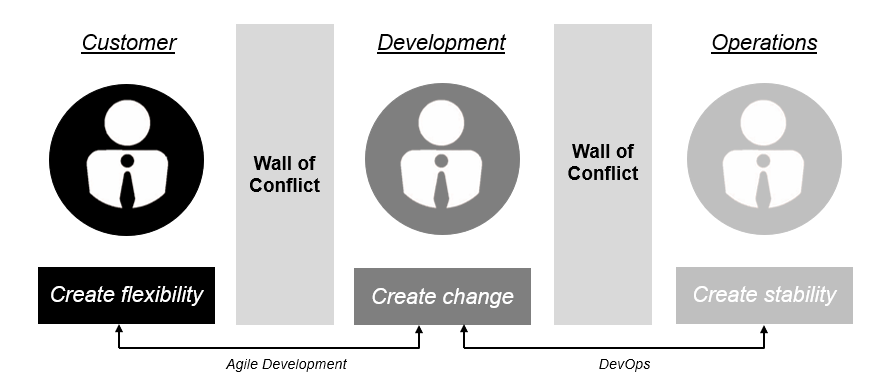
\includegraphics[scale=0.6]{Bilder/Wall of Conflict.png}
    \caption{Wall of Conflict, angelehnt an \cite{hering_devops_2018}}
\end{figure}

Gründe dafür waren, dass sowohl Entwickler- als auch Betriebsteam unterschiedliche Ziele, Denkweisen und Prozessen verfolgt haben. \cite{wettinger_streamlining_2016} Der daraus resultierende Engpass führte zu einem erheblichen Mehraufwand insbesondere im Bereich des Ops-Teams und zu verspäteten Auslieferungen von Softwareprojekten. Mittels des DevOps-Ansatzes sollen die Silos zwischen der Entwicklung des Betriebs aufgebrochen werden, indem kleine und funktionsübergreifende Teams gebildet werden, die die DevOps-Praktiken und Prinzipien verfolgen. \cite{ebert_devops_2016}, \cite{wiedemann_research_2019} In diesem Rahmen werden automatisierte Pipelines aufgebaut, um manuelle Arbeiten zu reduzieren und eine kontinuierliche Bereitsstellung sicherzustellen. \cite[S.3,5]{verona_practical_2016} Demnach sollte einerseits eine dauerhafte Interaktion mit dem Kunden stattfinden und andererseits keine Messung von großen Meilensteinen mehr erfolgen. \cite[S.5]{sharma_devops_2017}\\\\ Aus diesem Grundgedanken heraus, handelte es sich bei dem DevOps-Ansatzes zunächst um eine kulturelle Bewegung, die die Unterschiede zwischen Dev und Ops verändern sollte und die Bereitstellung mittels Automatisierung, schneller, effizienter und kontinuierlicher zu gestalten. \cite[S.5]{sharma_devops_2017} Letztlich kann DevOps nicht als ein vollständig neuer Ansatz, sondern vielmehr als eine Weiterentwicklung bereits bekannter Konzepte angesehen werden. \cite[S. 23]{alt_innovationsorientiertes_2017}



\subsubsection{Der Begriff 'DevOps'}
Wie bereits zu Anfang erwähnt, besteht der Kunstwort 'DevOps' aus den Begriffen Development und Operations. 

Grundsätzlich beschreibt dieses Konzept die Kombination zwischen der Entwicklung (Development) und dem Betrieb (Operations) als ein funktionsübergreifendes Team. 

Trotz detaillierter Prinzipien, die als Basis von DevOps gelten, findet sich keine einheitliche Standarddefinition zu diesem Begriff. \cite{sollner_devops_2017},\cite{smeds_devops_2015}

Je nach Zielsetzung, Unternehmenskultur oder Spezifikation werden in der Literatur viele Definitionen aufgelistet, in denen versucht wird, das Konzept des DevOps zu analysieren und zu beschreiben.

Diese Tatsache kann zuweilen daran liegen, dass ein großer Teil der verfügbaren Informationen über DevOps aus Blogs und anderen informellen Veröffentlichungskanälen stammen, die oftmals nicht glaubwürdig oder wissenschaftlich belegt sind. \cite{smeds_devops_2015},\cite{roche_roche_2011}

So führt beispielweise Hüttermann\cite[S. 3,4]{huttermann_devops_2012} aus, dass es keinen einheitlichen Begriff für DevOps gibt, der alle Aspekte von DevOps umfasst. 

Seiner Ansicht nach, werden durch die weite Verbreitung viele verschiedene Inhalte aus unterschiedlichen Perspektiven mit DevOps in Verbindung gebracht.

Gemäß Hüttermann beschreibt DevOps eine Mischung aus bekannten, forschrittlichen Praktiken und neuen, innovatioven Ansätzen für allgemeine Herausforderungen im Projektleben der Softwarebereitstellung und des Betriebs. 

Aufgrund der Vielschichtigkeit und der unterschiedlichen Fähigkeiten und Prioritäten, die sowohl Entwickler als auch Systemadministratoren besitzen, kann DevOps keine Berufsbezeichnung oder eine Abteilung innerhalb einer Organisationsstruktur sein. \cite[S. 9]{huttermann_devops_2012} 

In diesem Rahmen beschreiben Hüttermann\cite[S. 3,4]{huttermann_devops_2012} als auch Willis\cite{willis_what_2010} DevOps als Muster für die Zusammenarbeit, Prozesse und Tools, wobei Aspekte und Aktivitäten wie Kultur, Automatisierung, Messung und gemeinsame Nutzung umfasst werden.

Diese Kernelemente werden ebenfalls von Humble und Molesky \cite{humble_why_2011} als wesentliche Bestandteile einer DevOps-Umgebung beschrieben. 

Walls \cite[S.1]{walls_building_2013} hingegen ist der Meinung, dass DevOps eine kulturelle Bewegung ist, die mit einer Reihe von Softwareentwicklungspraktiken vermischt wird, die eine schnelle Entwicklung ermöglichen. 

Roche \cite{roche_roche_2011} geht davon aus, dass es zwei Standpunkte hinsichtlich einer Standarddefinition für DevOps gibt. 

Die erste Seite identifiziert ein spezifisches Berufsbild für DevOps, wobei Entwickler hauptsächlich am Code arbeiten, Systemadministratoren hauptsächlich mit Systemen arbeiten und DevOps eine Mischung aus diesen beiden Fähigkeiten ist. \cite{muller_whats_2010}

Die andere Partei erweitert die erste Auffassung und stellt allerdings klar, dass DevOps kein Job im herkömlichen Sinne ist. 

Mitglieder eines DevOps-Teams sind Entwickler mit etwas mehr Erfahrung und Wissen als ein Systemadministrator oder möglicherweise ein Systemadministrator mit etwas Erfahrung und Wissen als ein Programmierer. \cite{jones_how_2012}

Daher stellt DevOps eine Verschmelzung von Softwareentwicklung und Support für ein besseres Toolset zur Erkennung und Messung von Problemem in vernetzten Systemen dar und gilt nicht als ein Job der dazu beiträgt, einen neuen Standard für alle in der Softwarebranche zu definieren. \cite{roche_roche_2011} 

Jez Humble ein bekannter Autor, Mitbegründer der DevOps Research and Assessment LLC und Vordenker der DevOps-Bewegung, beschreibt DevOps als einen \textit{'movement of people who care about developing and operating reliable, secure, high performance systems at scale, has always — intentionally — lacked a definition or manifesto'} \cite{humble_state_2014}

Humbles Ansicht nach ist diese Tatsache jedoch nicht problematisch da die Auswirkungen von DevOps, der Beweiß dafür sind, in wieweit die DevOps-Praktiken und die DevOps-Kultur die IT- als auch die Unternehmensleistung, eine Organisation beeinflussen können. \cite{humble_state_2014}

Diese Auswirkungen wurden bis heute in dem jährlichen und 'DevOps Report' \cite{puppet_inc_2020_2021} veröffentlicht und beschreiben wie durch DevOps-gestützte Praktiken eine hohe organisatorische Leistung erzielt und im Ergebniss einen signifikanter Wettbewerbsvorteil erlangt wurde. 

In dieser Hinsicht bedeutet DevOps für Humbles nicht, dass sich ein Team für die Erstellung und Bereitstellung von Systemen, das Deploment oder den Betrieb dieser Systeme verantwortlich ist. \cite{humble_theres_2012}

Daher kann es keine Rollen für einen DevOps-Spezialisten in den Teams geben. 

Vielmehr erkennt DevOps Problemzustände und strebt ein strategisches Ziel, mit menschlichen, technischen und organisatorischen Lösungsansätzen, an. \cite{konig_devopswelcome_2019}\cite{dyck_towards_2015}

Aufgrund der Vielschichtigkeit und des unterschiedlichen Knowhows in dem DevOps-Umfeld wird in dieser Thesis ebenfalls die Ansicht von Hüttermann und Humble vertreten, dass DevOps kein Berufsbild im klassichen Sinne darstellt.

Daher wird die Definition von Penners und Dyck \cite{dyck_towards_2015} vertreten, in der DevOps als ein \textit{'an organizational approach that stresses empathy and cross-functional collaboration within and between teams – especially development and IT operations – in software development organizations, in order to operate resilient systems and accelerate delivery of changes.'} beschreibt. 

Darüber hinaus sind kulturelle Askpekte von zentraler Bedeutung innerhalb von einer DevOps-Umgebung, allerdings können diese nicht als Basis angenommen werden. \cite{smeds_devops_2015}

%Vielmehr baut ein DevOps-Team eine Plattform zur Nutzung und zur Bereitstellung für die gesamte Organisation auf. 

%Diese Plattform kann als ein Produkt angesehen werden, welches das Team als solches weiterentwickelt und die Personen die es nutzen, als Kunden angesehen werden können.

\subsubsection{Grundlagen}
Anhand des DevOps-Ansatzes wird eine Kultur oder Umgebung etabliert, durch die das Erstellen, Testen und Freigeben von Software schnell, häufig und zuverlässiger erfolgen kann. \cite[S.xxviii]{sharma_devops_2017} Obwohl die Gründe für die Einführung von DevOps vielschichtig sein können, sollen in erster Linie Ineffizienzen in den Softwareentwicklungs-, Release- und Betriebsprozessen vermieden werden, die durch die organisatorische Trennung zwischen den Prozessen \cite{lwakatare_devops_2019} oder durch die Fehlkommunikation zwischen den Teammitgliedern \cite{ebert_devops_2016} verursacht werden. Generell ist es für Teams innerhalb der Entwicklung nicht möglich, neue Softwareversionen freizugeben oder Softwareänderungen schnell vorzunehmen, wenn der Betrieb die jeweiligen Funktionen nur langsam bereitstellen kann. \cite[S. 7,8]{sharma_devops_2017} Vor diesem Hintergrund stehen die Bereiche der Entwicklung und des Betriebs oft im Zielkonflikt "Agilität vs. Stabilität" und sehen sich mit verschiedenen Hindernissen konfrontiert, darunter unbefriedigende Testumgebungen und schlechter Informationsfluss. \cite{lwakatare_devops_2019}, \cite[S. 8]{sharma_devops_2017}, \cite{konig_devopswelcome_2019} Die Folgen sind eine verspätete Bereitstellung von Releases, Fehler in den Releases oder eine fehlende Dokumentation. \cite[S. 24]{alt_innovationsorientiertes_2017} Hinzu kommen Probleme wie mangelndes Knowhow von Entwicklen über die Betriebnahme der verwendeten Systeme, fehlendes Vertrauen in den Ops-Bereich hinsichtlich der Stabilität, verzögertes Testen oder Verschwendung durch mangelnde Wiederverwendung von Quellcode. \cite{humble_why_2011}\\\\ Mittels DevOps sollen die Interessen aller Beteiligten ausglichen werden, mit besonderem Schwerpunkt auf Entwicklern, Testern und Betriebspersonal. \cite{humble_why_2011} Die querschnittlich aufgestellten Teams, lösen sich aus abgegrenzten Organisationseinheiten und Verantwortungsbreichen, aus den sogenannten 'Silos' und treiben gemeinsame Ergebnisse durch eine effektive Zusammenarbeit voran. \cite[S.5]{halstenberg_devops_2020}, \cite{sollner_devops_2017} Die daraus resultierenden Vorteile, reichen von einer schnelleren Produktbereitstellung, bessere Ressourcenauslastung und Automatisierung bishin zu einer stabileren Betriebsumgebung. 

\paragraph{2.1.3.1 CALMS} $~$
Generell lassen sich die Werte von DevOps, wie in Abbildung 2 dargestellt, in dem bekannten Akronym CALMS zusammenfassen: Kultur (Culture), Automatisierung (Automation), Schlankheit (Lean), Messung (Measurement) und Teilen (Sharing). 

\begin{figure}[h]
     \centering
     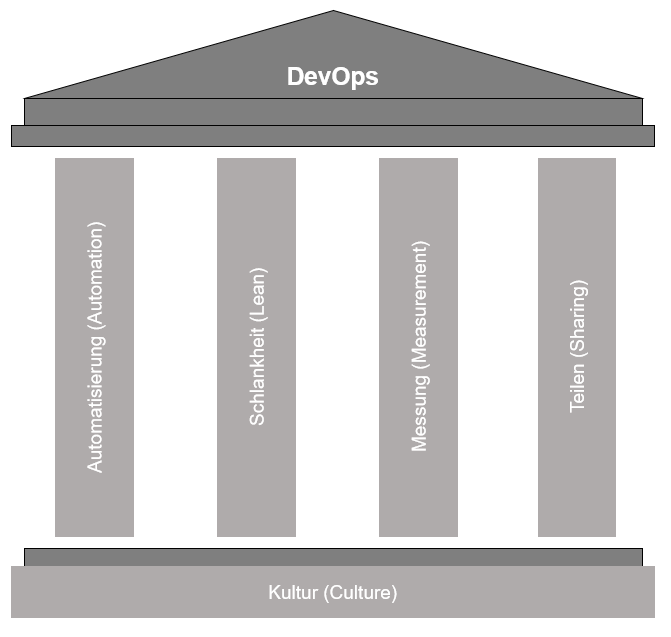
\includegraphics[scale=0.4]{Bilder/Calms.png}
     \caption{Die Säulen von DevOps, basierend auf dem CALMS-Prinzip, angelehnt an \cite{hornby_devops_nodate}}
 \end{figure}

Der Aspekt der Kultur beinhaltet zunächst die Ausrichtung nach dem Menschen. Hierbei spielt die Kollaboration als ein funktionsübergreifendes Team und die Orientierung nach Kundenwünschen eine tragende Rolle für eine DevOps-Organisation. \cite[S.5]{halstenberg_devops_2020} Die Automatisierung von Entwicklung, Implementierung und Tests ist der Schlüssel zum Erreichen niedriger Vorlaufzeiten und damit zu schnellem Feedback. \cite{humble_why_2011} 'Lean' steht in diesem Zusammenhang für die Vermeidung von Verschwendung jedlicher Ressourcen, Transparenz, ganzheitliche Betrachtung und Prozessoptimierung. Der Faktor der Messung orientiert sich an den messbaren Daten, um den Fortschritt eines Unternehmens zu begutachten. Die definierten und erhobenen Kennzahlen reichen dabei von den Verfügbarkeiten und den Zeiten für die Fehlerbehebung oder Codeänderungen bis zu den Zeiten für die Anforderungsänderungen. \cite[S. 7]{halstenberg_devops_2020} Die letzte Säule beschreibt das Teilen von Informationen, Wissen, Vorgehensweisen und Praktiken innerhalb eines oder zwischen verschiedenen Teams unterschiedlicher Abteilungen. \cite{halstenberg_devops_2020} Dabei soll eine Umgebung geschaffen werden, in der gegenseitige Austausch, die Kommunikation und die gemeinsame Nutzung im Vordergrund stehen.\\\\

Bei dem gesamten Vorteilen und Mehrwerten, die durch DevOps erreicht werden können, kann DevOps jedoch als kein Nullsummenspiel oder Selbstläufer gesehen werden. \cite{humble_why_2011} Der DevOps-Ansatz benötigt zunächst einen kulturellen Wandel, was eine große Herausforderung für viele Unternehmen darstellen kann. Standardisierte Herangehensweisen sind von einer Vielzahl von Unternehmen über die Jahre tiefgreifend verankert worden, wodurch Mitarbeiter ihre gewohnten Arbeitsabläufe anpassen müssten. Dies reicht von der Erlernung neuer Tools, Technologien und Methoden, Aufbau einer Kommunikation für den gegenseitigen Austausch, vollständige Automatisierung, Verschmelzung etablierter Rollen und Zuständigkeiten, Schwierigkeiten bei der Implementierung eines automatisierten Deployment-Prozesses oder die Übernahme neuer Aufgaben und Verantworlichkeiten. \cite{lwakatare_devops_2019}, \cite[S. 594 - 595]{abrahamsson_product-focused_2016}, \cite[S. 43 - 45]{halstenberg_devops_2020} Da sich die Bedeutung von DevOps in den letzten Jahren verschoben hat und immer wieder neue Tools für DevOps auftauchen, handelt es sich bei DevOps um eine stetige Weiterentwicklung. \cite[S. 595]{abrahamsson_product-focused_2016} Daher gibt es keinen Standard fester Praktiken im Zusammenhang mit DevOps, wodurch sich nicht festlegen lässt, welche Praktiken für DevOps eingesetzt werden sollten. 


% Insgesamt soll das Ziel verfolgt werden, die Softwarebereitstellung kontinuierlich sicherzustellen um so reaktionschnell auf Veränderungen am Markt oder Kundenanforderungen reagieren zu können.

%Die Trennung zwischen Projekten und Betrieb ist zu einer schwerwiegenden Einschränkung geworden, einerseits für die Fähigkeit von Unternehmen, neue Funktionen schneller auf den Markt zu bringen, andererseits für die der IT, stabile und qualitativ hochwertige Systeme und Dienste zu warten. \cite{humble_why_2011} 

%Ersetzen von Softwareentwicklungsmethode durch Kultur, Bewegung oder Praxis.
%Hinzufügung des Hinweises auf Automatisierung

%In diesem Abschnitt werden die grundsächlichen Merkmale von Devops beschrieben. Zudem werden wesentliche Vorteile beschrieben, durch die die Integration von DevOps möglich sind. Des weiteren wird auf das CALMS-Modell (Culture, Automation, Lean, Measurement und Sharing) eingegangen.

%DevOps gilt nicht als ein Nullsummenspiel, indem die Bereitstellungen häufig und zuverlässig in einer stabilen Produktumgebung erreicht werden, sondern es ist ein Ansatz zur Behebung der genannten Probleme durch Kultur, Automatisierung, Schlankheit, Messung und gemeinsame Nutzung, welches auch als CALMS bekannt ist. \cite{humble_why_2011



% Die Abbildung 2 zeigt den chronischen Konflikt, der oftmals innerhalb der IT-Organsisation herrscht, der durch fehlende Interaktion zwischen diesen Bereichen enstehen, die häufig unterschiedliche Ziele und Prozesse verfolgen. \cite[S. 349 - 350]{kim_devops-handbuch_2017}

% \begin{figure}[h]
%     \centering
%     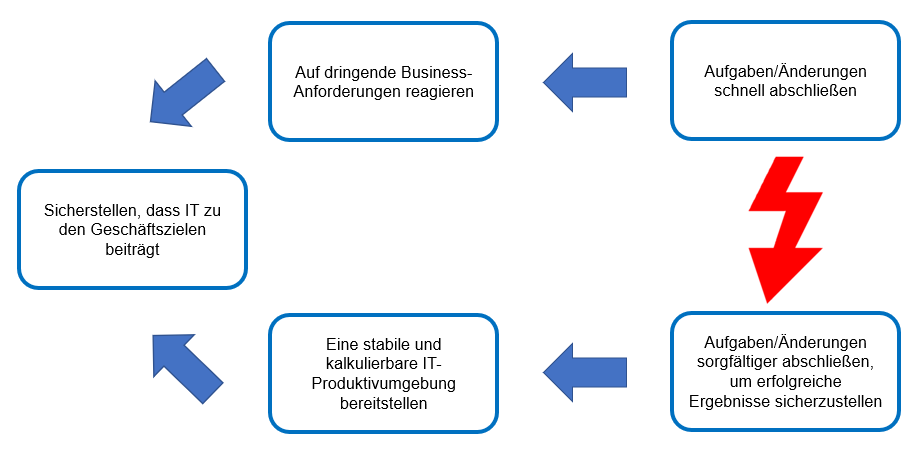
\includegraphics[scale=0.6]{Bilder/Core Conflict Clouds}
%     \caption{Zentraler chronischer Konflikt nach Gene Kim \cite[S. 349]{kim_devops-handbuch_2017}}
% \end{figure}
% \dwi{irgendwie hab ich das gefühl diese grafik "läuft" in die falsche richtung.}

\subsubsection{DevOps-Kultur}
Durch die intensive Interaktion der Bereiche Entwicklung und Betrieb müssen unterschiedliche organisatorische und kulturelle Veränderungen durchgeführt werden, damit die DevOps-Kultur etabliert werden kann. 

In diesem Rahmen baut DevOps auf den Hauptprinzipien, als das Model der \textit{'The Three Ways'} auf, die von dem Autor Gene Kim \cite{kim_devops-handbuch_2017} definiert wurden. 

Dieses Model der drei Wege bilden die zugrunde liegenden Prinzipien von DevOps ab, indem das Verhalten und die Muster von DevOps näher beschrieben werden. \cite[S. 9 - 11]{kim_devops-handbuch_2017}, \cite{kim_three_2012}  

Der erste Weg bildet die Grundlage für DevOps ab und betont die Leistung des gesamten Systems, im Gegensatz zur Leistung eines besitmmten Teams oder einzelner Abteilungen. 

Der Fokus liegt auf einem schnellen Arbeitsfluss, der durch die IT ermöglicht wird. 

Den Anfang stellt die Entwicklung dar, über die Operations bis hin zum Kunden.

Dabei wird das Produkt, basierend auf den identifizierten Anforderungen, von der Entwicklung erstellt und in den Betrieb übergeben, wo dies dem Kunden ausgeliefert wird. 

Während dieses Schrittes sind alle Arbeiten sichtbar und in kleinen Aufgaben aufgeteilt, die in bestimmten Intervallen ausgeführt werden. 

In diesem Rahmen wird versucht, mehrere Ziele zu erreichen. 

Zunächst sollte das Verständnis des Arbeitssflusses sichergestellt werden. 

Unabhängig um welche Arbeit es sich handelt, sollte diese stillstehen oder zu einem negativene Ergebnis führen, ist dies fast immer ein Hinweis auf Probleme, die gelöst werden müssen. 




Zu den Ergebnissen der Umsetzung des Ersten Weges in der Praxis gehört, dass niemals ein bekannter Fehler an nachgelagerte Arbeitsplätze weitergegeben wird, dass eine lokale Optimierung niemals zu einer globalen Verschlechterung führt, dass immer versucht wird, den Fluss zu erhöhen, und dass immer versucht wird, ein tiefes Verständnis des Systems zu erlangen (im Sinne von Deming).


%Durch die Interaktion der beiden Bereiche Development und Operations gehen auch organisatorische Änderungen mit einher, damit eine umfassende DevOps-Kultur geschaffen werden kann. In diesem Abschnitt wird insbesondere auf die Ziele dieser Kultur eingegangen, damit die Zusammenarbeit zwischen den beiden Bereichen gelingt. In diesem Rahmen wird unter anderem auf die wesentlichen Aspekte/Werte wie Kontniuierliches Lernen, Experimentieren, Ingenieurskultur, Kultur der Effektivität, Produktdenken oder die Übernahme von Verantwortung eingegangen. Auch wird der Vergleich und die Nachteile des traditionellen Silodenkens aufgegriffen. 

\subsubsection{Entwicklungszyklus innerhalb DevOps}
Der DevOps-Lebenszyklus besteht aus mehreren iterativen und meist automatisierten Workflows, die innerhalb eines größeren, iterativen und automatisierten Zyklus ausgeführt werden \cite[S. 16]{halstenberg_devops_2020}. Grundsätzlich baut der Entwicklungszyklus innerhalb einer DevOps-Umgebung auf sieben Phasen auf, wie in der Abbildung 2.6 zu erkennen ist. 

\begin{figure}[h]
    \centering
    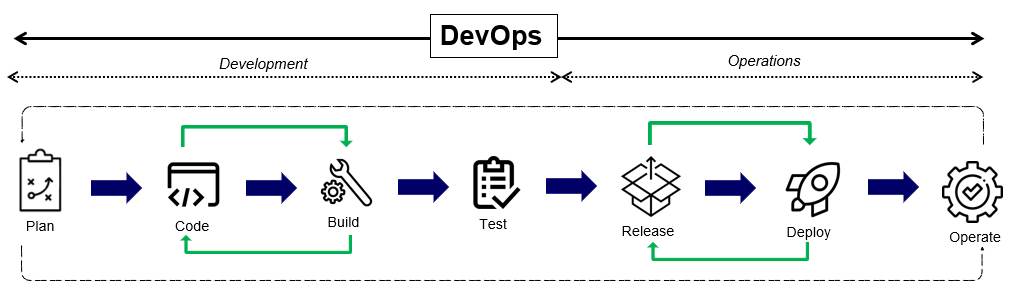
\includegraphics[scale=0.6]{Bilder/DevOps Lebenszyklus.png}
    \caption{Entwicklungszyklus innerhalb einer DevOps-Umgebung, angelehnt an \cite[S. 16]{halstenberg_devops_2020}}
\end{figure}

Der Zyklus verläuft stets in einer Schleife, wodurch sich sowohl der Prozess als Ganzes als auch die einzelnen Phasen, untereinander durchgehend wiederholen, um eine stetige Neuimplementierung, Weiterentwicklung, Zusammenarbeit und Feedback sicherzustellen. Aufgrund der Iteration des Zyklus können Fehler in den einzelnen Phasen frühzeitig erkannt und beiseitigt werden und tragen zur Verbesserung der gesamten Phase bei. Die Tätigkeitsfelder von Dev und Ops verbinden sich, wobei jedes Tätigkeitsfeld seperate als auch zusammenarbeitende Aufgaben erfüllt, mit dem Ziel, die Geschwindigkeit, Zuverlässigkeit und die Qualität des Prozesses zu gewährleisten. 

\subsubsection{2.1.5.1. Plan}$~$

In dieser Phase werden zunächst die wesentlichen Anforderungen, Problembeschreibungen und der Entwicklungsumfang anhand der Bedürfnisse aller Stakeholder oder durch erhaltenes Feedback festgelegt, mit dem Ziel, die Entwicklung und die Auslieferung entsprechend zu planen \cite[s. 16]{halstenberg_devops_2020}. An dieser Stelle kommen Methoden der agilen Softwareentwicklung wie Scrum, Kanban oder Extreme Programming zum Einsatz. Durch die Planung und Koordination mittels Kanban-Board können nicht nur reine Entwicklungstätigkeiten, sondern auch Schwerpunkte im Hinblick auf den Betrieb zur Infrastruktur oder Wartung als Arbeitsschritt abgebildet werden \cite{schaefer_devops_2017}. Zur kurzfristigen Kontrolle können die auf Scrum basierenden Planungsgrundsätze verwendet werden, da dieses auf zeitlich begrenzte Iterationen und die Verteilung von Rollen und Zuständigkeiten setzt. Wichtige Gemeinsamkeit beider Methoden ist die Arbeit nach dem Pull-Prinzip, wobei Tasks eigenständig bearbeitet werden, wenn die entsprechende Kapazität zur Verfügung steht \cite{concas_agile_2007}. Ferner können sich Entwickler einen Überblick über die Verwendung von Systemen, Features, Funktionalitäten Risiken und Einschränkungen verschaffen \cite{yarlagadda_devops_2021}. 

\subsubsection{2.1.5.2. Code und Build} $~$

Nachdem die wesentlichen Aufgaben zugewiesen worden sind, stellt die hauptsächliche Aktivität innerhalb dieser Phase die Entwicklung dar. Schritte wie beispielsweise das Testen, die Inbetriebnahme oder die Berücksichtigung der Anfoderungen sollten in dieser Phase bereits berücksichtigt sein \cite[S. 18]{halstenberg_devops_2020}. Die Forschritte des zu entwickeltenden Programmcodes werden laufend in Sprint Reviews oder Daily Scrum Meetings an das gesamte DevOps-Team kommuniziert. Um eine einheitliche Basis zu schaffen, arbeiten alle Entwicklerteams mit gemeinsamen Tools und Plugins und legen einheitliche Vorgaben für die Qualität des Quellcodes fest. Zudem werden alle Veränderungen am Programmcode, neue Entwicklungen oder Fehleranfälligkeiten dokumentiert und für das gesamte DevOps-Team zur Verfügung gestellt.

\subsubsection{2.1.5.3. Test} $~$

Während dieser Phase werden intensive Tests der Anwendungen und Funktionalitäten innerhalb einer eigenen Serverumgebung durchlaufen, die auch als 'Staging Environment' bezeichnet werden \cite[S. 16]{verona_practical_2016}. Dabei wird eine Umgebung geschaffen, die sich ähnlich der Produktionsvariante verhält, auf die die finale Version bereitgestellt wird und daher ein Testen unter annährend realen Bedingungen erlaubt \cite[S. 5.2/5.6]{bass_devops_2015}. Durch die Verwendung von realen Daten sollen Funktionaliäten unabhängig von der Entwicklungsumgebung, anhand der Infrastruktur geprüft und simuliert werden \cite[S. 16]{verona_practical_2016}. Während Entwicklerteams Unit- und Integrationstests durchführen, beteiligt sich der Betrieb an Integrations- und Lasttests, um die Betriebsbereitschaft zu beurteilen \cite[S. 127]{sturm_devops_2017}. Neben den automatisierten Tests finden darüber hinaus auch manuelle Tests statt, um Schwachstellen oder Risiken in Bereichen wie Sicherheit innerhalb der Anwendung zu identifizieren und zu beseitigen.

\subsubsection{2.1.5.4. Release und Deploy} $~$

Die Phase des Release beschreibt den Prozess der Vorbereitung für die Bereitstellung des Builds an entwickelten Funktionalitäten in die produktive Umgebung \cite[S. 20]{halstenberg_devops_2020}. In diesem Zuge können neue Versionen innerhalb fester Zeiträume erfolgen oder automatisiert, nach erfolgreicher Übergabe des Quellcodes durch die Testphase \cite{thedev_eight_2019}. Abhängig von dem Fortschritt des Release-Prozesses kann die Übergabe sowohl manuell als auch automatisiert und ohne Einschränkungen des laufenden Betriebs erfolgen, wobei Entwickler, Funktionalitäten deaktivieren können bis diese einsatzbereit sind \cite{thedev_eight_2019}. Bei Problemen innerhalb des Deployments, kann der letzte Stand aus der Produktivumgebung wiederhergestellt werden, indem die neue Umgebung parallel zur bestehenden Produktionsumgebung aufgebaut wird. Häufig kann die Phase des Deploys mit der Phase des Releases übereinstimmen, obwohl diese Phase im Wesentlichen nur die Auslieferung der getesteten Software in die Produktivumgebung beschreibt \cite[S. 20]{halstenberg_devops_2020}.

\subsubsection{2.1.5.5. Operate} $~$

Diese Phase beschäftigt sich hauptsächlich mit der Wartung und den Support, nachdem die Änderungen live gegangen sind. In diesem Rahmen werden einerseits Lastspitzen oder Tiefpunkte anhand der aktiven Nutzerzahl automatisiert und effektiv abgefangen und andererseits benötigte Ressourcen zur Verfügung gestellt, um die Produktivumgebung erfolgreich zu betreiben \cite{thedev_eight_2019}. Häufig wird als finale Phase, die Monitor-Phase zusätzlich in den DevOps-Lebenszyklus aufgenommen, wobei diese oftmals in die Operate-Phase mitaufgenommen werden kann. Zudem kann der Kunde Feedback geben, welches gesammelt und ausgewertet wird, um die Erhebung von weiteren Daten wie den auftretenden Fehlern, Leistungsverhalten, Zugriffszahlen oder Kapazitäten \cite{thedev_eight_2019}. Durch die erhobenen Informationen kann sichergestellt werden, dass der aktuelle Zustand einer Anwendung überwacht und verwaltet wird, um sich auf Änderungen vorzubereiten und etwaige Fehler zu beheben \cite[S. 127]{sturm_devops_2017}.

















 







% Im Rahmen von Scrum werden zunächst alle am System zu erledigenden Arbeiten im 'Release Backlog' festgehalten. 

% Während der Planung für den Sprint werden Features und Funktionen aus dem Release Backlog ausgewählt und in das 'Sprint-Backlog' oder nach Prioritäten gesetzten Aufgaben aufgenommen, die im nächsten Sprint abgeschlossen werden sollen. \cite{cohen_introduction_2004}

% Infoldessen können mögliche Entwicklungsaufwände auf einen zeitlichen Umfang versehen ('Timeboxing'). \cite[s. 17]{halstenberg_devops_2020}

% Die Organisation des Teams findet in kleinen Sitzungen und monatlichen Sprints oder Iterationen statt. 

% Während Scrum sich auf die iterative Produktentwicklung konzentiert und das Produkt von Teration zu Iteration erweitert und verbessert, arbeitet die Kanban-Methode auf die kontinuierliche Verbesserung der Prozesse, kürzere Vorlaufzeiten und Vermeidung von Verschwendung, hin. \cite{concas_agile_2007}

% Zudem legt Scrum den aktuellen Arbeitsfortschritt und die Planung auf die folgenden Sprints fest, während sich die Planung bei Kanban auf mehrere Wochen bezieht. \cite[s. 5]{verona_practical_2016} 
% Insbesondere die messbaren und eindeutigen Vorteile von DevOps zeigen sich innerhalb kürzerer Zyklen, die wiederum die längeren Zyklen effizienter machen. 





% Diese Vorgehensweise wird auch als Push bezeichnet, der wiederrum einen Pull-Request auslöst. 

% In diesem Zusammenhang erfolgt ein Code-Review, bei dem der Pull-Request bestätigt wird sobald der Quellcode den Anforderungen funktional entspricht.

% Analog zum Pull-Request finden automatisierte Testfälle und die (ausführbare) Konfguration der Test- und Produktionsumgebung statt. \cite[S. 18]{halstenberg_devops_2020}  

% Ist das Testen erfolgreich durchlaufen, kann der Quellcode übernommen werden. 

% Nachdem die Aufgabe abgeschlossen ist, wird der neu entwickelte und lauffähige Programmcode in kleinen Bestandteilen an ein Versionsverwaltungstool ('Repository') übergeben.\cite[S. 18]{halstenberg_devops_2020} 



% Neben der Entwicklungsphase erfolgt innerhalb der DevOps-Zyklen eine intensive Testphase, die in einer eigenen Umgebung durchgeführt wird und sich vor den Phasen der Intergration und der Bereitstellung befindet. 



% m Rahmen dieser Phase sind zwei grundlegende Rollen verbreitet. \cite[s. 20]{halstenberg_devops_2020} 

% Zum einen trifft der Release Coordinator die Entscheidungen über den Produktiveinsatz eines Releases und überwacht den Entwicklungsfortschritt. 

% Zum anderen überwacht der Site Reliability Engineer die IT-Services, die notwendigen Tools und Abhängigkeiten innerhalb der Inbetriebnahme des Releases. 




%Nun wurde die Idee hinter dem DevOps-Ansatz wird in den vorherigen Kapiteln beschrieben. Als nächstes soll nun näher auf die inhaltlichen Themen von DevOps eingegangen werden, sowie der DevOps Life Cycle und dessen Phasen. Damit der Life Cycle nicht zu weitgreifend wird, wird lediglich der Life Cycle, der bei der msg systems ag verwendet wird, näher beschrieben. Damit sollte der Leser ein Verständnis für die weiteren Punkte im Proof Of Concept erlangen.\\




%Gemäß Fluri u.a. \cite[S. 259 - 283]{tokarski_strategische_2018} muss ein optimaler DevOps-Prozess drei Voraussetzungen erfüllen, um erfolgreich etabliert zu werden. Erste Voraussetzung bilden zunächst die \textit{automatisierten und definierten Prozesse}. Um Prozesse optimiert und effizient zu etablieren und zu automatisieren, bedarf es zunächst einer umfassenden Definition über die Funktionsweise und den Ablauf dieses Prozesses. Hinzu kommt eine \textit{integrierte Infrastruktur(Toolchain)}. Anhand technischer Komponenten als geeignete Werkzeuge, die dem DevOps-Team zur Verfügung gestellt werden, kann die Automatisierung optimal abgebildet werden. Letzte grundsätzliche Voraussetzung stellt das \textit{Rahmenwerk von Aktivitäten für die Teams} auf. Diese Voraussetzung zielt auf die Etablierung einer DevOps-Kultur, die bereits im vorherigen Kapitel dargestellt wurde. Gemäß Fluri u.a. \cite[S. 259 - 283]{tokarski_strategische_2018} wird der gesamte Entwicklungszyklus in DevOps durch acht Schritte und vier Prozessgebiete abgebildet. 





\subsubsection{Continuous Everything als DevOps-Methoden}
Während sich agile Praktiken im Hinblick auf die Softwareentwicklung auf eine kontinuierliche Planung, Flexibilität und eine schnelle Reaktion auf sich ändernde Kundenanforderungen fokussieren, können DevOps-Praktiken dazu verwendet werden, den Arbeitsfluss vom Kunden über die Entwicklung, den Betrieb und zurück kontinuierlich auszubauen und damit die Qualität und Belastbarkeit der Software zu steigern. \cite{fitzgerald_continuous_2014} \cite[S. 264]{tokarski_strategische_2018}

Die \textit{'Continuous Everything'}-Methoden spiegeln die Idee einer kontinuierlichen Verbesserung und Automatisierung innerhalb eines Devops-Prozesses wieder. 

Wie in der Abbildung zu erkennen ist, können sich diese Methoden auf merhrere Entwicklungszyklenphasen konzentrieren und werden in diesem Abschnitt im Einzelnen beschrieben.  

\begin{figure}[h]
    \centering
    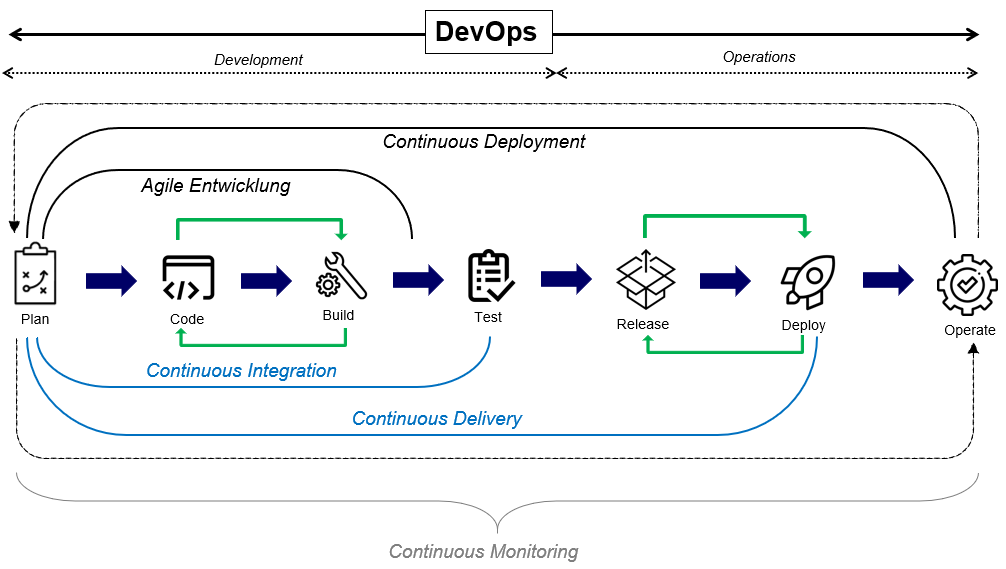
\includegraphics[scale=0.6]{Bilder/Continuous Everything.png}
    \caption{Continuous-Methoden innerhalb des Devops-Lebenszykluses, angelehnt an \cite[S. 16]{halstenberg_devops_2020}}
\end{figure}

\paragraph{Agile Entwicklung}
\dwi{ich glaube das brauchst du hier nicht nochmal ausdetaillieren.}
Die agile Entwicklung beschreibt die Verwendung von agilen Methoden innerhalb des Softwareentwicklungsprozesses als eine wesentliche Grundvoraussetzung für den DevOps-Prozess. 

Oftmals wird dieser Prozess auch als Continuous Planning (dt kontinuierliches Plannen) bezeichnet und reicht von der Phase des Planes bis zur Phase des Builds. \cite{fitzgerald_continuous_2014} 

Wie bereits in der Phase des Planens beschrieben, können agile Methoden wie Scrum und Kanban zum Einsatz kommen um die entsprechenden Ressourcen und die Entwicklungen während des ganzen Zeitraums zu planen und einzuteilen.

Inerhalb dieser Methode werden Features in kleinen Inkrementen geplant und entwickelt, um diese innerhalb eines Sprints umzusetzen und folglich die Durchlaufzeit bis zur Auslieferung kurzzuhalten. \cite[S. 266]{tokarski_strategische_2018} 

Infolgedessen beinhalten die Ergebnisse dieser Methode ausliefbare und getestete Funktionalitäten nach jedem Sprint. 

Continuous Planning gilt als ein ganzheitliches Unterfangen, dass ein engere Intergration zwischen Planung und Ausführung erfordert und an dem sowohl Kunden als auch die Entwickler beteiligt sind. \cite{fitzgerald_continuous_2014} 

Ziel ist es sicherzustellen, dass die Investitionsentscheidungen während des gesamten Lbenszykluses auf die Bedürfnisse des Kunden abgestimmt worden sind. 

\paragraph{Continuous Integration}
\dwi{diese abschnitte sind sehr relevant, weil du später ja auch konkret in diesen aspekten erweiterungen im Vorgehen definierst. hier lohnt es sich wahrscheinlich, aspekte die du als hintergrund für deine anpassungen brauchst insbesondere hervorzuheben.}
Die Methode des Continous Integration (dt. kontinuierliche Integration, kurz: CI) beschreibt grundsätzlich die Gewährleistung einer sicheren und lückenlosen Integration von Codeänderungen in die vorhandenen Umgebungen. \cite[S. 266]{tokarski_strategische_2018}  

Ziel ist es, die Qualität der Software sicherzustellen und schnelles Feedback über die Integrierbarkeit vor der Auslieferung zum Kunden zu erhalten. \cite[S. 266]{tokarski_strategische_2018} 

Kernelement stellt ein Versionsverwaltungssystem (auch: Repository) dar, dessen wesentliche Aufgabe es ist, den DevOps-Teams dabei zu helfen, den Code von mehreren Entwickeln zu organisieren, Änderungen zu verfolgen und automasierte Tests zu ermöglichen. 

Zunächst werden neuer oder geänderter Code nach der Entwicklung und Prüfung regelmäßig und in möglichst kurzen Abständen in einem gemeinsamen Repository gemergt (dt. zusammengeführt). \cite[S. 13-16]{sharma_devops_2017}

In diesem Zuge wird der Code automatisiert in einem Build kompiliert. 

Die neu erstellten Artefakte, als Ergebnis des Builds, werden in eine lauffähige Umgebung integriert und automasiert getestet. 

Damit soll sichergestellt werden, ob die neue Codeänderung einer Komponente im Kontext der gesamten Anwendung lauffähig ist. 

Dies ist essentiell für den Prozess, da häufig viele Entwickler an der Codebasis mit leicht unterschiedlichen Versionen arbeiten und daher überprüft werden kann, ob die verschiedenen Änderungen richtig zusammenarbeiten. \cite[S. 69]{verona_practical_2016} 

Aufgrund des regelmäßigen Integrieren der Codeänderungen wird gewährleistet, dass häufige automatisierte Tests durchführt werden, den Entwicklern stets der aktuellste Code zur Verfügung steht und Entwickler nicht darauf warten müssen, einzelne Codeabschnitte am Tag der Veröffentlichung auf einmal zu integrieren. \cite{thedev_eight_2019} 

Durch die entstehende Flexibilität und Geschwindigkeit können Fehler schneller und leichter behoben werden, da die Programmbestandteile kleiner und weniger komplex sind und das Debugging insgesamt sinkt. \cite{thedev_eight_2019}

Darüber hinaus werden Änderungen sichtbarer und bilden eine starke Grundlage für zukünftige Änderungen. 

Insgesamt umfasst CI Schritte wie die Codekompilierung, die Durchführung von Unit- und Akzeptanztests, die Validierung der Codeabdeckung, die Überprüfung der Einhaltung von Codierungsstandards und die Erstellung von Bereitstellungspaketen. \cite{fitzgerald_continuous_2014} 

\paragraph{Continuous Delivery}

Da regelmäßig Builds durch die Continuous Integration erzeugt werden, müssen diese zeitnah in andere Umgebungen weitergeleitet werden. \cite[S. 16 - 18]{sharma_devops_2017}  

Bei dem Ansatz des Continuous Delivery (dt. kontinuierliches Ausliefern, kurz: CD) handelt es sich um die nächste Stufe des Continuous Integration. 

Die Methode des Continuous Delivery baut auf einer regelmäßigen und automatisierten Bereitstellung des Builds an den Testbereich, zur anschließenden Bewertung und zu einer potentiellen Freigabe an die Kunden, auf. \cite[S. 16 - 18]{sharma_devops_2017}  

Voraussetzung ist der Aufbau einer Continuous-Delivery-Pipeline, zum Ziel das Ausrollen der Software möglichst automatisiert für die Bereitstellung neuer Releases durchzuführen. \cite[S. 10]{wolff_continuous_2016}

Sobald ein neues Artefakt innerhalb des Repositorys übertragen wurde, wird die Continuous-Delivery-Pipeline ausgelöst. \cite[S. 14]{verona_practical_2016} 

In diesem Rahmen werden die fehlerfreien Builds automasiert innerhalb eines produktionsähnlichen Staging- oder Testbereich bereitgestellt, um nach dem Testen zu bewerten, wie sich die Builds produktionsnah verhalten und letztlich in die Produktion verlagert werden können. \cite[S. 16]{sharma_devops_2017}

Falls das Testen in der Pipeline fehlschlägt, werden die Entwickler informiert und haben dmait die Gelegenheit kurzfristig Anpassungen an dem jeweiligen Build vorzunehmen oder diesen zu verwerfen. 

Insgesamt soll sichergestellt werden, dass die neu entstandene Version für den Einsatz im Produktivbetrieb geeignet ist. \cite{thedev_eight_2019}

Das Versionieren in Releases und das Ausliefern der Software wird bei Continuous Delivery möglichst vollständig durch geeignete Tools automatisiert. 

Die Methode des Continuous Delivery beinhaltet mehrere Vorteile für das gesamte DevOps-Team. 

So wird aufgrund des hohen Grades an Automatisierung der Release-Prozess maßgeblich verbessert, indem Risiken und Engpässe durch die häufige Auslieferung von kleinen Features vermieden werden können und damit ein kontinuierlicher Integrationsfluss sichergestellt werden kann. \cite[S. 18]{wolff_continuous_2016}

Zudem sind die Test- und Release-Phasen der Pipeline abgestimmt und ermöglicht es Unternehmen, das Release neuer Builds in beliebigen Abständen manuell auszulösen. \cite{thedev_eight_2019}

\paragraph{Continuous Deployment}

Die letzte Phase der Delivery-Pipeline ist das Continuous Deployment (dt. kontinuierliche Bereitstellung, kurz: CD).

Kernaufgabe des Continuous Deployments ist die voll automatisierte Überführung des Codes in die Produktivumgebung mithilfe der Delivery-Pipeline. \cite[S. 29]{alt_innovationsorientiertes_2017} 

Sowohl Continuous Delivery als auch Continuous Deployment werden in der Literatur oftmals synonym verwendet, da beide auf analoge Konzepte basieren. 

Der Unterschied zwischen beiden Methoden besteht darin, dass Continuous Deployment ein automatisiertes Ausliefern der neuen Version auf die Produktivumgebung beinhaltet, während Continuous Delivery die Auslieferung auf nicht-produktive Umgebungen abzielt. 

Demnach kann das Deployment auf die Produktivumgebung im Rahmen des Continuous Delivery manuell entschieden werden, die widerrum von den fachlichen Erfordernissen des Kunden abhängt. \cite[S. 29 - 30]{alt_innovationsorientiertes_2017} 

Aufgrund der automatisierten Freigabe des Releases, muss sowohl die Qualität als auch die Lauffähigkeit der Pipeline besonders gesichert sein, was wiederrum in der Phase des Continuous Delivery gewährleistet sein muss. \cite[S. 269]{tiemeyer_handbuch_2021} 

Continuous Deployment entspricht demnach der höchsten Stufe einer Delivery-Pipeline, was den DevOps-Teams ermöglicht, kleinste Features und Änderungen für den Anwender ausliefern zu können und wäre theoretisch das höchste Ziel der modernen Softwareentwicklung. \cite{humble_why_2011}  

Durch den höchsten Grad der Automatisierung können die Vorlaufzeiten niedrig gehalten und folglich schnelles Feedback erhalten werden. \cite{humble_why_2011}   

Das Ziel ist es demnach, die Zeit bis zur Markteinführung von der Software zu verkürzen, indem jeder Commit in die Produktivumgebung bereitgestellt wird. 

Viele Entwickler und Unternehmen lehnen die Methode des Continuous Deployments jedoch ab, da es ein Risiko darstellt, wenn eingecheckter Code durch das Testing fehlgeschlagen ist, automasiert in die Produktivumgebung bereitgestellt wird. \cite[S. 269]{tiemeyer_handbuch_2021}  

Um dieses Risiko möglichst gering zu halten, müssen einerseits nahezu produktionsreife Codes und robuste Test-Frameworks vorhanden sein und andererseits alle DevOps-Mechanismen zuverlässig arbeiten. \cite[S. 269]{tiemeyer_handbuch_2021}  

Darüber hinaus verlangt der Continuous-Deployment-Ansatz eine starke Architekturaufsicht und Teamdisziplin, damit das Release nicht die Qualität oder den von den Kunden realisierten Nutzen in Mitleidenschaft zieht.\cite[S. 119 - 120]{erder_continuous_2016} 

An diesem Punkt ist es wichtig, eine Kultur des Vertrauens aufzubauen, die die Zusammenarbeit aller Teamsmitglieder fördert. \cite{humble_why_2011} 

\paragraph{Continuous Monitoring}
\dwi{hm dieser und folgende punkte sind zum einen nicht in der grafik oben, auf die du dich ja (sehr konsistenterweise, gut!) stützt. hier kann man wieder über den fokus/rotstift nachdenken..}
Die Vorgehensweise des Continuous Monitoring umfasst die durchgängige Überwachung, der zugrunde liegenden Infrastruktur und des im Betrieb befindlichen Quellcodes. \cite{van_hoorn_continuous_2012} 

Dabei stellt das Ops-Team sicher, dass die Anwendung in der Produktion funktioniert wie gewünscht und die Umgebung stabil läuft. 

Hierfür haben die Ops-Teams eigene Tools zur Überwachung ihrer Umgebung und laufenden Systeme und zwar von der Prozessebene bis hinunter zu Ebenen, die niedriger sind, als es die Systemüberwachungstools erlauben würden. \cite[S. 26]{sharma_devops_2017}

Oftmals werden Selbstüberwachungs- und Analysefunktionen direkt in die zu entwickelnden Anwendungen eingebaut, um eine kontinuierliche End-to-End-Überwachung zu gewährleisten. \cite[S. 26]{sharma_devops_2017}

Neben der Anwendungs- und Systemleistung muss das Benutzerverhalten der Anwendung und die Benutzerzufriedenheit ebenfalls überwacht werden, um ein detalliertes Feedback zu erhalten. \cite[S. 112 - 113]{erder_continuous_2016}

Dieses Feedback kann schnell in die Phase der Entwicklung zurückfließen, um bessere Entscheidungen bei der Entwicklung der nächsten Änderung treffen zu können. 

Auf diese Weise können zusätzliche und neue Anforderungen und Funktionen berücksicht, Probleme behoben und das weitere Vorgehen angepasst werden. 

Sowohl das Feedback als auch Fehler, Probleme oder Ausfälle werden anhand einer Feedbackschleife zurück an die Entwicklung kommuniziert und im besten Fall möglichst zeitnah behoben. \cite[S. 112 - 113]{erder_continuous_2016} 

Im Ergebnis bildet diese Feedbackschleife ein Instrument, zur kontinuierlichen Gestaltung und Orientierung für das Softwareprodukt.   

\paragraph{Infrastructur-as-a-Code}

Automatisierung gilt als eine Grundvoraussetzung innerhalb der Devops-Umgebung und erstreckt sich nicht nur auf die Bereiche der Entwicklung und Bereitstellung, sondern auch auf die zugrundeliegende Infrastruktur. \cite[S. 272]{tiemeyer_handbuch_2021} 

Insbesondere durch die Verwendung von Continuous Integration, ist die Anzahl der Umgebungen und ihrer Instanzen stark angestiegen, da täglich Builds getestet, validiert und bei Konfigurationsänderungen angepasst werden müssen. \cite[S. 19]{sharma_devops_2017}

Obwohl die Vorgehensweise des \textit{Infrastructur-as-a-Code} (kurz: IaC) keine 'Continuous'-Bezeichnung besitzt, ist diese Praktik wesentlicher Bestandteil der gängigen DevOps-Methoden. \cite[S. 30]{alt_innovationsorientiertes_2017} 

Anstatt manuelle Änderungen durch einen Administrator, welcher schrittweise ein neues System einrichtet oder umkonfiguriert, werden Ressourcen, Netzwerkeinstellungen, Parameter und weitere Konfigurationen als Code in einer Konfigurationsdatei beschrieben. \cite{juner_praxisbasierte_2017} \cite{luber_was_2020}

Genau wie bei dem Quellcode für die Software, wird der Code für die Infrastruktur innerhalb eines Versionsverwaltungssystem registriert und in einem Repository zur Verfügung gestellt.

Damit kann der Aufbau einer Infrastrukturumgebung automatisiert aufgebaut und bereits bei der Entwicklung miteinbezogen werden.

Durch die entstehende Versionierung sind alle Änderungen überprüfbar, reproduzierbar und bei Fehlern können Rollbacks auf die frühere Version durchgeführt werden.\cite[S. 272]{tiemeyer_handbuch_2021}   

\textit{Dadurch kann jeder produktivähnliche Umgebungen in Minuten erhalten, ohne ein Ticket aufmachen oder gar Wochen warten zu müssen.} \cite[S. 107]{kim_devops-handbuch_2017}

Voraussetzung für IaC ist es, Systemadministratoren frühzeitig innerhalb des Softwareentwicklungsprozesses einzubeziehen und das Verständnis der Entwickler für die auf dem Produkt basierende Infrastructur zu schärfen, wodurch die Zusammenarbeit der Bereiche Dev und Ops verbessert wird. \cite[S. 30]{alt_innovationsorientiertes_2017}

Mittels IaC würde die alleinige Verantwortung für alle Phasen wie das Design, Umsetzung, Test, Installation und Betrieb bei einem DevOps liegen. \cite{kasteleiner_devops_2019}

Aufgrund der steigenden Automatisierung der Pipeline als auch durch IaC werden die Umgebungen immer identischer, was widerrum dem Grundgedanken des Continuous Integration entspricht, da der Quellcode sehr früh auf eine produktionsnahe Umgebung integriert wird und dadurch Probleme schnell sichtbar werden. \cite[S. 111 - 113]{kim_devops-handbuch_2017} 


\subsubsection{Integrierte Infrastruktur (Toolchain)}
Insbesondere aufgrund der immer größer werdenden Komplexität eingesetzter Technologien für den Softwareentwicklungs- und Deployment-Prozess, ist die Automatisierung im DevOps-Umfeld ein essentieller Bestandteil. Durch einen hohen Grad an Automatisierung sollen wiederholende Aufgaben reduziert werden, mit dem Ziel das Risiko manueller Fehler zu vermeiden und die Verschwendung von menschlichen Ressourcen zu minimieren. Gemäß des DevOps-Konzepts werden die Grundsätze des DevOps-Ansatzes durch den Aufbau einer Bereitstellungspipeline (engl. Deployment Pipeline) durchgesetzt. Die Deployment-Pipeline besteht im Wesentlichen aus mehreren Continuous Integration und Continuous Delivery-Pipelines und kann als eine automatisierte Implementierung der Build-, Test-, Deployment- und Release-Prozesse einer Anwendung definiert werden. \cite{humble_why_2011} Insbesondere die Testautomatisierung ist ein zentraler Bestandteil der Deployment Pipeline. Während zu Beginn einfache Unit-Tests ausreichen, müssen mit fortschreitender Automatisierung zur Sicherstellung der Qualität und Lauffähigkeit Funktions-, Last- oder Integrationstests implementiert werden, bis ein manuelles Testen bestenfalls überflüssig wird. \cite[S. 27]{alt_innovationsorientiertes_2017}, \cite[S. 110 - 111]{wolff_continuous_2016} Eine entsprechende Deployment-Pipeline kann durch den Einsatz passender Tools (dt. Werkzeuge)etabliert werden und stellt mit Hilfe miteinander kombinierter Tools eine optimale Abdeckung der Automatisierung sicher. \cite[S. 268]{tokarski_strategische_2018} Werden die Deployments automatisch in die Produktivumgebung ausgeführt, sind die DevOps-Teams ab diesem Zeitpunkt in der Lage, jederzeit eine neue Funktion, Fehlerbehebung oder Anpassungen an der Infrastruktur, auszuliefern. \cite{juner_praxisbasierte_2017} Wesentliche Ziele der Deployment-Pipeline sind, einen End-to-End-Prozess für alle sichtbar zu erstellen und durch die frühe Problemerkennung und -behebung das bestehende Feedback zu verbessern. \cite[S. 3 - 4]{humble_continuous_2011} In der Abbildung 8 wird die Deployment-Pipeline schemenhaft dargestellt und im Folgendem, anhand der Intergrations- und Delivery Pipeline näher erläutert.  

\begin{figure}[h]
    \centering
    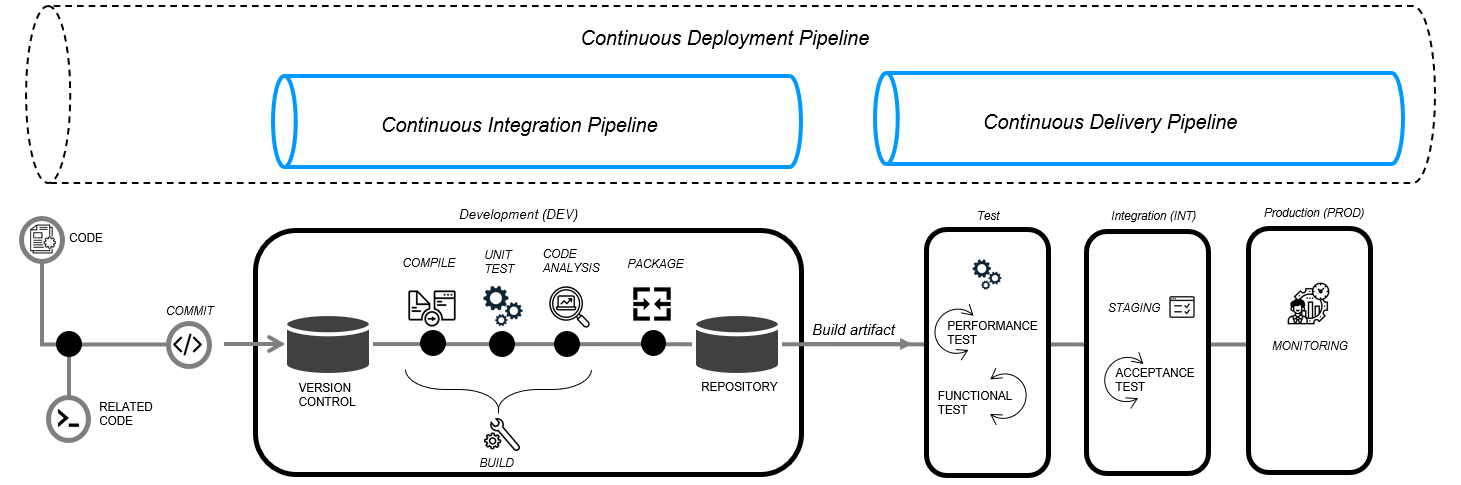
\includegraphics[scale=0.4]{Bilder/Continuous Deployment Pipeline.png}
    \caption{CD-Pipeline, angelehnt an \cite{balajee_what_2020}, \cite[S. 17]{sharma_devops_2017}}
\end{figure}

\paragraph{2.1.7.1. Integration Pipeline} $~$

Wie in der Abbildung 8 zu sehen ist, wird die Continuous Integration Pipeline zunächst bei jedem Einspielen von Code Commits automasiert angestoßen, wodurch der Code kompiliert wird und alle Unit-Tests durchgeführt werden. \cite[S. 266]{tokarski_strategische_2018}. Dabei erfolgen Unit-Tests automatisiert und ermöglichen ein schnelles Testen des Verhaltens von kleinen vorgenommenen Codeänderungen isoliert von den anderen Komponenten der Software. \cite[S. 60]{humble_continuous_2011} Nachdem das Testen erfolgreich abgeschlossen wurde, wird der Commit angenommen und die statische Analyse des Quellcodes kann beginnen. \cite[S. 61]{verona_practical_2016} Diese liefert Informationen über den Zustand des Codes, über Defekte, Design-Probleme oder ob Schwachstellen in den Bibliotheken von Drittanbietern gefunden wurden. \cite[S. 61]{verona_practical_2016}\\\\ Wichtige Voraussetzung für die Integration der CI-Pipeline ist zunächst die Verwendung einer Versionskontrolle. \cite[S. 100 - 101]{bass_devops_2015}, \cite[S. 57]{forsgren_mindset_2019} Diese ermöglicht es einzelnen Entwicklern, unabhängig von ihrem Standort oder von der Funktion, an der sie arbeiten, parallel zusammenzuarbeiten und sofort kleine Änderungen an dem Code zu erfassen. \cite[S. 57]{humble_continuous_2011} Um automatische Tests und Zusammenspiel aller Funktionen auf dem integrierten Master-Branch sicherzustellen und zeitaufwendige Code-Merges zu vermeiden, müssen insbesondere Feature-Branches bei der Entwicklung kurz gehalten werden. \cite{meyer_continuous_2014} Folglich soll die gesamte Entwicklung der Features in einem Branch in der Versionskontrolle und nicht auf dem Master-Branch stattfinden, wodurch die Entwickler an einem bestimmten Feature arbeiten können, ohne die Codebasis innerhalb des Master-Branches zu behindern. \cite[S. 44 - 45]{verona_practical_2016} Sobald Änderungen mit dem Main-Branch zusammengeführt werden, werden diese in automatischen Build-Prozessen und mittels Tests validiert. Nach der Validierung des Quellcodes wird dieser innerhalb eines Intergrationsservers (CI-Server) als ein Build erstellt in einem Repository veröffentlicht. Bei Änderungen des Builds werden erneut Unit-Tests durchgeführt, um die Funktionalität der Anpassung sicherzustellen. \cite[S. 57]{forsgren_mindset_2019} 


\paragraph{2.1.7.2. Delivery Pipeline} $~$

Die Continuous Delivery Pipeline erweitert die CI-Pipeline, um die erfolgreich durchgeführten Builds automatisch in produktionsähnlichen Testumgebungen bereitzustellen, in denen funktionale Test, Integrationstests und Performance-Tests durchgeführt werden. \cite[S. 17]{sharma_devops_2017} Wie in der Abbildung 8 dargestellt, ist der Auslöser für die CD-Pipeline jedes neue Build-Artefakt, welches im Repository veröffentlicht wird. Zusätzlich zum Quellcode werden alle Build-Artefakte innerhalb des Repositorys gespeichert, während die gleichen Versionen für die Entwicklungs-, Test- sowie Produktionsumgebung verwendet werden. \cite[S. 109 - 110]{kim_devops-handbuch_2017} Im nächsten Schritt wird der Code zusammen mit der entsprechenden Konfiguration, als ein Artefakt Build, also eine ausführbare Anwendung gebaut und sollte ab diesem Zeitpunkt nicht mehr verändert werden. In diesem Rahmen führt der CI-Server systemübergreifende Integrationstests an dem jeweiligen Build auf der Integrationsumgebung vor, um die fehlerfreie Interaktion der gesamten Komponenten miteinander zu testen. \cite[S. 122]{kim_devops-handbuch_2017} Während der Integrationstest wird eine Anbindung zu einer Testdatenbank konfiguriert, die aus einer ausreichenden Menge von Daten besteht, um die mit der Integration verbundenen automatisierten Tests durchzuführen. \cite[S. 100 - 101]{bass_devops_2015} Als nächsten Schritt wird die Software innerhalb der Staging-Umgebung, als eine produktionsähnliche Umgebung testweise betrieben, ohne die Interaktion der produktiv betriebenen Services. \cite[S. 100 - 101]{bass_devops_2015} Anschließend erfolgen die Akzeptanztests, die mit einer Anzahl von Nutzern festgelegte Use Cases der Anwendung testen und direktes Feedback über Schwachstellen oder funktionale Probleme liefern. \cite[S. 16 - 18]{sharma_devops_2017} Ferner können die Akzeptanztests auch automatisiert eingesetzt werden, was wiederrum den Grad der Wiederholbarkeit erhöht. Im Anschluss werden nicht-funktionale Tests und Performance-Tests durchgeführt.\\\\ Im besten Fall wird der Build durch die CD-Pipeline automatisch in die Produktivumgebung bereitgestellt, vorausgesetzt alle Tests wurden erfolgreich bestanden, anderenfalls wird das Deployment gestoppt und das Team wird über den Zustand des Builds informiert. \cite[S. 64]{forsgren_mindset_2019} Nachdem die Anwendung auf den normalen Produktivumgebung bereitgestellt wird, läuft diese konstant in einer Version oder aus einer Kombination von mehreren Versionen (Microservices). \cite[S. 86]{kim_devops-handbuch_2017} Die Architektur des Microservices bildet die Grundlage für den DevOps-Ansatz und beschreibt den Aufbau von Anwendungen, basierend auf eine große Anzahl an kleinen Services. \cite{sollner_devops_2017} Diese Services bestehen aus kleinen separaten funktionalen Codeteilen, die miteinander interagieren und miteinander ein Anwendungssystem abbilden. Oftmals wird nur eine Funktionalität abgebildet und kommuniziert mit anderen Services über eine definierte Schnittstelle. Mittels Microservices lassen sich einzelne Funktionalitäten leicht und schnell deployen und anpassen, wodurch das gesamte Deployment erhöht, die Wartung vereinfacht und das restliche System nicht gefährdet wird. \cite[S. 85 - 86]{kim_devops-handbuch_2017} Dieser Ansatz vereinfacht die Methode des Continuous Integration.

% Insgesamt lässt sich die Continuous Deployment Pipeline als einen automatischen, regelmäßigen Prozess der Bereitstellung erfolgreicher Builds in die Produktivumgebung beschreiben.

%Frage an Daniel: 
%1. Feature-Toggling, verschiedenes Testing (A/B-Tests, Canary-Tests, Live Test oder Beta-Tests), oder das Blue/Green Deployment erwähnen/beschreiben/erklären?????
%2. Irgeendwie bin ich mir nicht sicher, bei der Kapitelüberschrift---> Idee?



% Insbesondere die Testautomatisierung ist ein zentraler Bestandteil der Deployment Pipeline, da jede neue Version eines Builds über mehrere Schritte getestet, wiederholt getestet und anschließend an die Produktivumgebung übergeben werden muss.

% Um die Rolle der Automatisierung voranzutreiben, werden möglichst viele vollautomatisierte Deployments auf die Produktivumgebung aufgesetzt. 




 











  











 








%Working: Last step, tbd
\subsection{OSS}
\centering

\includegraphics[scale=0.7]{Bilder/what-is-foss}

\subsubsection{Entwicklungen und Unterscheidungen von Software}
\subsubsection{Freiheiten als Merkmale von FOSS}
\subsubsection{Nutzungsrechte an FOSS}
\subsubsection{Lizenzarten und Lizenzmodelle für FOSS}
\subsubsection{Urheberrechtliche Aspekte}
\subsubsection{Vertragrechtliche Aspekte}
\subsubsection{Kritische Betrachtung bei der Verwendung von FOSS}



\section{OSS meets DevOps}
Nachdem der theoretische Rahmen und die Funktionsweise beider Bereiche beschrieben worden ist, wird in diesem Kapitel näher auf die Integration der OSS innerhalb des Prozesses der DevOps-Produktentwicklung, eingegangen.

In den letzten Jahren hat sich die Nutzung der OSS über die Jahre als ein Standard in der Softwareentwicklung innerhalb Unternehmen etabliert. 

Die Gründe sind verschiedenartig und reichen von Innovationskraft, Flexibilität, Geschwindigkeit bis zur Reduzierung der Kosten.

Zunächst können die Reduzierung der Gesamtkosten als ein essentieller Grund für die Verwendung von OSS-Komponeten angesehen werden. 

Im Gegensatz zu proprietärer Software wird OSS kostenlos heruntergeladen und kann je nach Anforderungen angepasst werden. 

Zwar fallen in der Regel auch mit Verwendung von OSS zusätzliche Kosten für Schulungen, Wartung und Support an, wobei diese als \emph{sunk costs}




Der offensichtlichste Vorteil von Open-Source-Software ist, dass die Produkte in der Regel kostenlos heruntergeladen werden können, wobei sie mit Betriebskosten wie etwa für Speicher und Rechenleistung verbunden sind. Selbst die seltenen kostenpflichtigen Open-Source-Produkte sind in der Regel immer noch viel günstiger als Closed-Source-Alternativen.

Die Einführung von Open-Source-Software hat in der Regel geringere Vorlaufkosten (da die Software oft kostenlos oder relativ kostengünstig ist) und verlagert die Kostenstelle von der Lizenzierung (Betriebskosten) auf die Anpassung und Implementierung (Investitionskosten). Zusätzliche Kosten wie Schulung, Wartung und Support sind „sunk costs“. Unternehmen zahlen dafür, unabhängig davon, ob es sich bei der Software um Open Source oder Closed Source handelt. Insgesamt stellt sich heraus, dass Open Source sicher und effizient genug ist sowie insgesamt kostengünstiger.






In derselben Studie wurden auch die wichtigsten Vorteile untersucht. Am wichtigsten ist zumindest Unternehmen und Behörden in der Schweiz die Unterstützung von offenen Standards, wie sie der Europäische Interoperabilitätsrahmen für eGovernment
definiert. An zweiter Stelle steht der Kontakt zur Community, die meist bei Fragen zur Software hilft und so
einen Enterprise Support ersetzen kann. Erst an dritter Stelle liegen Einsparungen z.B. durch fehlende Lizenzkosten. Direkt danach folgt die Unabhängigkeit von proprietärer Software, die teilweise mit den genannten Einsparungen verknüpft sind.
Die Studienautoren führen an, dass geschlossene Software mit “geschlossene[n] Datenformate[n], die technisch an Anwendungen gebunden sind; Lizenzvereinbarungen, die restriktiv wirken und die Flexibilität z.B. bei Wechseln einschränken und
Upgrade-Druck auslösen können” [2] Eigenschaften hat, die vielen Organisationen ein Dorn im Auge sind. Viele Software-Unternehmen haben dies auch erkannt und veröffentlichen ihre Software unter einer Open Source-Lizenz, damit sie beispielsweise nicht mit Microsoft Windows ausgeliefert werden oder andere Monopole unterstützen müssen. Weitere Vorteile bestehen in der stetigen Weiterentwicklung der Software, die zu einer höheren Sicherheit, einer höheren Stabilität und stetiger Innovation führt.











Allerdings fehlt in den meisten Unternehmen oftmals eine Strategie für die Nutzung und den Einsatz von OSS. 

\textit{Beliebtheit und zunehmende Verwendung stehen nach wie vor in Kontrast zu
einer grundsätzlichen Unkenntnis: So selbstverständlich die Verwendung ist, so verbreitet sind
oft auch Wissenslücken über Grundanforderungen im Umgang mit OSS, sei es als Basis für einen
erfolgreichen Einsatz im Alltag oder als Voraussetzung für die Verwendung für eigene Softwareprojekte.} \cite{bitkom_ev_open_2016}

Insbesondere im DevOps-Umfeld ist Verwendung von OSS-Komponeten mit wenig Hürden verbunden, wobei die Konsequenzen von den damit verbundenen Lizenzmodellen nicht jedem bewusst sind. 

Generell bedarf die Verwendung von OSS-Komponeten eine Schulung in Hinblick auf eine gewissenhafte Nutzung mit inkompatiblen Softwarelizenzen. 
















%In diesem Rahmen wird insbesondere auf drei Szenarien, die die Hauptanwendungsbereiche, der msg systems ag darstellen, näher beschrieben. 

\subsection{Gründe für die Einbindung von OSS}
\input{GründeEinbindungOSS.tex}

\subsection{Integration von OSS in die DevOps-Produktentwicklung}
Eine große Herausforderung bei der Modellierung des Softwareentwicklungsprozesses war eine genaue Momentaufnahme eines kontinierlichen arbeitenden Prozesses. 

\begin{figure}[p]
    \centering
    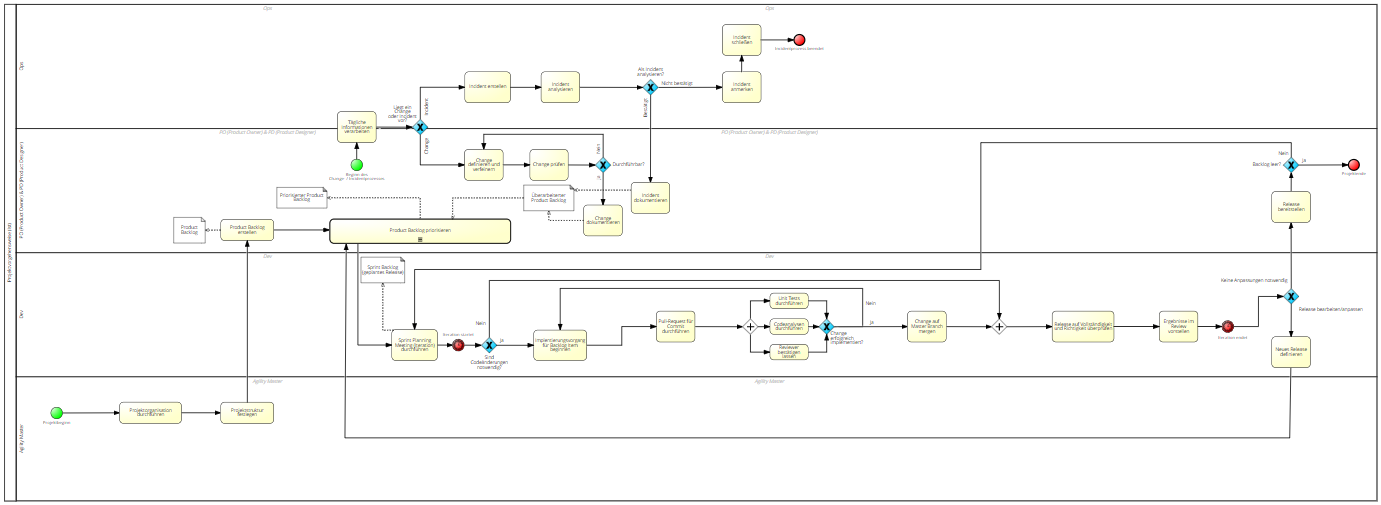
\includegraphics[angle=90, scale=0.7]{Bilder/IST-Prozess.png}
    \caption{Softwareentwicklungsprozess im IST-Zustand basierend auf dem HAF-Projekt}
\end{figure}

Da das DevOps-Team mit agilen Methoden wie Scrum und Kanban arbeitet, erwies sich die Modellierung des IST-Prozesses basierend auf einem Sprint am geeignesten. 

Der Prozess wurde zunächst in vier essentielle Rollen unterteilt, die bei der Softwareentwicklung als DevOps-Team beteiligt sind: 

\paragraph{Agility Master}

Der Agility Master verantwortet einen effektiven und effizienten Prozess und stellt sicher, dass die Regeln des agil und Lean Management eingehalten werden. 

Ferner fungiert der Agility Master als ein Moderator für Team-Ereignisse und versucht Probleme und Hindernisse zeitnah zu lösen. 

Der Agility Master ist mit dem Scrum Master identisch. 

\paragraph{Dev}

Diese Rolle entspricht der Rolle des Softwareentwickler oder Development-Teams. 

Je nach Projektanforderungen kann sich die Rolle des Entwicklers beispielsweise auf das Frontend- oder Backendentwicklung richten.

\paragraph{Product Owner und Product Designer}

Zunächst fungiert der Product Owner als die Schnittstelle zwischen verschiedenen Stakeholdern oder Kunden und dem Entwicklungsteam. 

Er vertritt demnach die Interessen des Kunden in den Entwicklungsprozess, ohne aktiv in die Softwareentwicklung einzugreifen.

Ferner erstellt der Product Owner den Product Backlog und legt die Reihenfolge der Items, die bearbeitet werden müssen, fest. 

Wie der Name schon sagt, beschreibt die Rolle des Product Designers die Gestaltung oder den Entwurf des Produkts. 

Hierzu gehören die Definitionen von UX-Anforderungen und Spezifikationen oder die Schaffung von Schnittstellen, im Hinblick auf die Fuktionalität und das erwartende Verhalten des Produkts. 

Innerhalb des HAF-Teams überschneiden sich die Rollen des Product Owner und des Product Designers, weshalb diese beiden Positionen in einer Swimlane dargestellt werden.  

\paragraph{Ops}

Die Rolle des Administratoren oder IT-Betrieb entspricht dem anderen Teil des DevOps-Teams. 

In erster Linie sorgt diese Rolle für die Stabilität der IT-Infrastruktur und ermöglichen einen durchgängigen, laufenden Betrieb.  

\begin{figure}[h]
    \centering
    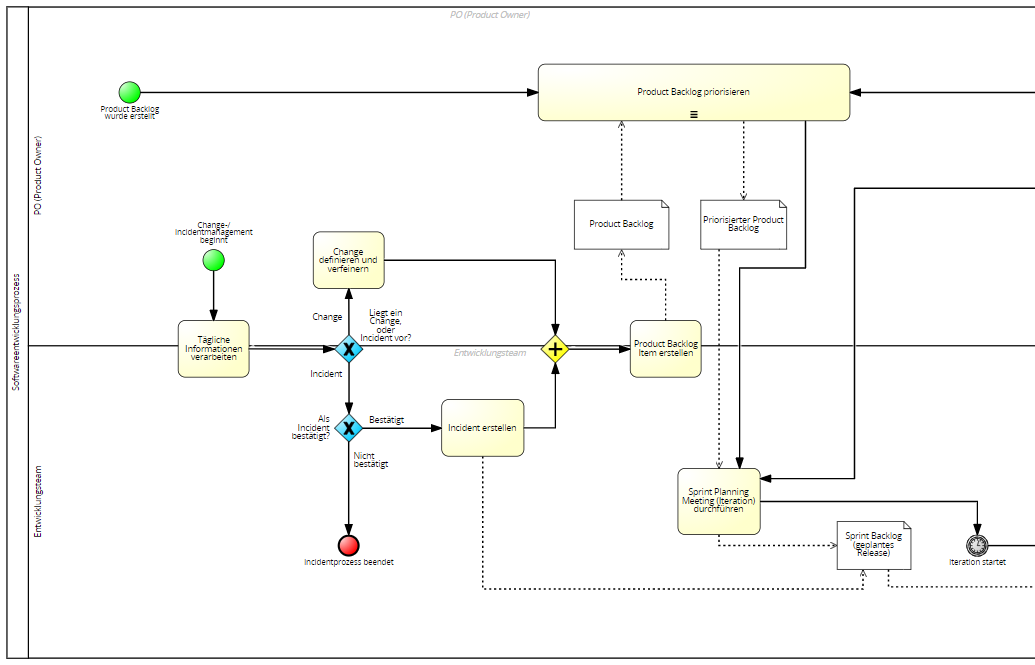
\includegraphics[scale=0.7]{Bilder/IST-Prozess_first Part.png}
    \caption{Erster Teil des Softwareentwicklungsprozess im IST-Zustand basierend auf dem HAF-Projekt}
\end{figure}

\newpage Startpunkt des Prozesses liegt beim Agility Master, indem die Projektorganisation zunächst durchgeführt und die Projektstruktur festgelegt wird.

Zu beachten ist, dass diese zwei Aufgaben ausschließlich am Anfang eines jeden Projekts und nicht in laufenden Projekten stattfinden. 

Nachdem das Product Backlog erstellt wurde muss dieses vom Product Owner priorisiert werden. 

Die Priorisierung findet sequentiell statt, da mehrere Entwicklungen und Änderungen eines Items des Product Backlogs parallel und gleichzeitig und nicht als eine Aufgabenschleife stattfinden. 

Diese Änderungen fließen in den priorisierten Backlog ein. 

Ist die Priorisierung erfolgt, startet die Iteration mit dem Sprint Planning Meeting. 

Abhängig von den verfügbaren Kapazitäten und den Ergebnissen des letzten Sprints wird entschieden, welche User Stories zuerst bearbeitet werden. 

Die ausgewählten User Stories bilden den Sprint Backlog. 

Parallel zu den täglichen Entwicklungen beginnt der Change-/Incidentprozess, bei dem zunächst die täglichen Informationen verarbeitet werden. 

Der Changeprozess bescheibt den prozess für eine Änderung, die sich auf eine geplante Modifikation der Definition eines bestehenden oder neuen Produkts bezieht und für die das DevOps-Teams verantwortlich ist. 

Der Prozess umfasst die Erfassung jedes Requests, die Dokumentation, Genehmigung und Kontrolle und stellt sicher, dass Change Requests definiert, geplant, effizient, wirtschaftlich und mit vertretbarem Risiko abgewickelt werden. 

Ein Ziel des Change Managements ist es, die Nachvollziehbarkeit von Anforderungen und Änderungen zu gewährleisten.

Incident Management umfasst den gesamten organisatorischen und technischen Prozess für Reaktionen und Maßnahmen auf Störungen des IT-Betriebs.

Das Spektrum möglicher Incidents reicht von Fehlermeldungen durch Anwender bis hin zu automatisierten Alarmen und Warnungen durch das Monitoring.

Das Ziel des Incident Managements ist die Wiederherstellung eines zugesagten Dienstes in einem definierten Prozess und in optimaler Zeit. 

Dies kann auch Umgehungslösungen beinhalten. 

Incident Management deckt keine (neuen) Anforderungen, Wünsche, Anfragen oder ähnliches ab.  

Obwohl der Change- und Incidentprozess vom Product Owner bzw. Designer begonnen wird, ist dieser ausschließlich für den Changeprozess verantwortlich. 

Der Incidentprozess wird anhand des täglichen Monitorings vom Ops-Verantwortlichen durchgeführt. 

Nach der Verarbeitung der täglichen Informationen, werden die auftretenden Bugs zunächst in Incident und Changeprozesses unterschieden, da beide Prozesse werden unterschiedlich behandelt werden.

Innerhalb des Changeprozesses werden die Änderungen definiert und verfeinert. 

Nachdem die Änderung geprüft wurde, muss entschieden werden, ob die Änderung durchführbar also entwickelt werden kann. 

Ist dies der Fall wird die Änderung dokumentiert und fließt in den überarbeiteten Product Backlog ein, bei dem die Items wiederrum innerhalb des Product Backlogs priorisiert werden. 

Sollte der Change nicht durchzuführen sein, müssen die Definitionen und Verfeinerungen angepasst werden.

Innerhalb des Incidentprozesses wird der Incident zunächst erstellt und analysiert.

Sollte der Bug als Incident bestätigt werden, so wird dieser dokumentiert und fließt in das überarbeitete Product Backlog und wiederrum in das priorisierte Product Backlog ein. 

Falls dies nicht der Fall ist, wird der Incident angemerkt und geschlossen, wodurch der Incidentprozess ab diesem Zeitpunkt geschlossen wird. 

Sobald die Iteration startet, muss zunächst überprüft werden, ob Codeänderungen notwendig sind. 

Dies kann sich auf Änderungen eines vorhandenen Codes oder auf eine Neuimplementierung beziehen. 

Sobald keine Änderungen notwendig sind, bleibt das entsprechende Item im priorisierten Product Backlog und wird im Release auf seine Vollständigkeit und Richtigkeit überprüft.

Nachdem der Pull-Request für das Commit durchgeführt wurde, werden mehrere Aufgaben parallel erledigt. 

Dazu gehört die Durchführung der Unit-Test und Codeanalyse und die Bestätigung des Reviewer.

Sobald alle Änderungen erfolgreich implementiert worden sind, werden diese auf das Master Branch gemergt. 

Sobald das Release auf seine Vollständigkeit und Richitgkeit überprüft worden ist, wird dieses im Review vorgestellt. 

Ab diesem Zeitpunkt endet die Iteration. 

Werden weitere Anpassungen benötigt, muss das neue Release bearbeitet und definiert werden, wobei diese in das priorisierte Backlog zurückgehen.

Sind keine Änderungen notwendig, wird das Release bereitgestellt. 

Das Projekt endet sobald das product Backlog leer ist.

















\subsection{Umfang der Integration anhand festgelegter Szenarien}
Um das Themenfeld der Verwendung von OSS in den Kontext des DevOps-Prozess innerhalb des HAF-Projektes in einem festen Rahmen erfassen zu können, musste zunächst der Umfang dieser Problemstellung reduziert werden.  

In diesem Rahmen wurde der Grad der Nutzung von OSS, insbesondere im Hinblick auf die Lizenzmodelle auf drei Szenarien beschränkt. 

Diese stellen zunächst drei Ausgangssituationen dar, unter welchen Bedinungen OSS innerhalb des konkreten HAF-Projekes verwendet werden dürfen und welche Einschränkungen dabei getroffen werden müssen.   

\paragraph{Szenario 1: Verwendung von OSS zur Testzwecken}

Bei dem ersten Szenario beschränkt sich die Nutzung von OSS ausschließlich auf Unterstützung- oder Testzwecke wie bespielsweise Treiber. 

Dementsprechend soll dieses Szenario verdeutlichen, dass die Verwendung von OSS ausschließlich als Werkzeug fungiert und keine Abhängigkeit zwischen der Funktionalität und der verwendeten OSS-Komponente stattfindet. 

Würde die OSS wegfallen, wäre die Funktionalität des Projekts weiterhin gewährleistet. 

Ferner werden keine Kopien des Original-Quellcodes innerhalb eines Repositorys hochgeladen, sowohl manuell als auch mittels Skript. 

Infolge der ausschließlichen Unterstützungsfunktion erfolgt innerhalb dieses Szenarios keine Auslieferung der Komponete an den Kunden. 

Demzufolge muss bei der Konstellation dieses Vewendungszwecks keine Beachtung der Lizenzmodelle genommen werden. 

\paragraph{Szenario 2: Verwendung von OSS-Bibliotheken als Referenz}

Im Rahmen des zweiten Szenarios wird der Quellcode der OSS während des Builds und Deployments heruntergeladen, um die ausführbare Datei zu erstellen. 

Damit können wiederverwendbare Software-Komponenten, welche generische Funktionalitäten des über festgelegte Schnittstellen bereitstellen, zeitnah eingebunden werden.

Zweck des zweiten Szenarios ist es, die OSS als reine Bibliothek zu verwenden und daher vollständig unverändert beizubehalten. 

Obwohl die Bibliothek ausschließlich unmodifiziert verwendet wird, ist sie Teil der ausführbaren Datei, welche beispielsweise über ein Artefakt-Feed bereitgestellt wird. 

Es entsteht demnach eine direkte Verbindung zu einer lizensierten OSS. 

Aus diesem Grund sollten innerhalb dieses Szenarios weitgreifend auf OSS-Komponenten mit einem starken Copyleft vermieden werden. 

\paragraph{Szenario 3: Verwendung von OSS als modifizierter Quellcode}

Innerhalb des letzten Szenarios findet eine tatsächliche Integration und Modifikation der OSS innerhalb der Entwicklung des Projekts statt.

In diesem Rahmen wird der Quellcode heruntergeladen, entsprechend den Anforderungen angepasst und letztlich in das Repository hochgeladen. 

Dies kann sowohl auf eine reine Modifikation des Quellcodes oder die Erstellung neuer Dateien basieren.  

Ab diesem Zeitpunkt ist die Berücksichtigung der Lizenzmodelle essentiell, wodurch bestimmte Bedinungen erfüllen werden müssen. 

Um weitgreifende Folgen zu vermeiden, sollten in diesem Szenario auschließlich OSS verwendet werden, die kein Copyleft oder teilweise ein beschränktes Copyleft aufweisen.

Jede Datei, welches modifiziert oder neu erstellt wurde, muss zur Kennzeichnung einer Modifikation mit einem Header-Kommentar versehen werden.

%Frage an Daniel: Szenarios grafisch darstellen?????

\subsection{Vorteile der Integration}
\input{VorteileIntegration.tex}

\subsection{Wesentliche Hindernisse}
\input{HindernissIntegration.tex}


\section{Proof of Concept}
Während die manuelle Checkliste dafür verwendet wird, präventiv OSS-Komponenten mit riskanten Lieznzmodellen bereits zu Beginn des Entwicklungsprozesses zu vermeiden, soll die automatisierte Checkliste das Ziel verfolgen, bereits implementierte OSS-Komponenten auf ihre Lizenzmodelle zu prüfen, bevor diese ausgeliefert werden. 

Diese wird innerhalb des folgenden Kapitels als der Proof of Concept (PoC) näher beschrieben. 

Grundsätzlich bestimmt der PoC die Machtbarkeit einer Idee, also ob die Idee wie geplant funktioniert und in die Realität umgesetzt werden kann, bevor für diese Ressourcen auf Produktionsebene verschwendet werden.  

In dem Rahmen dieser Arbeit stellt der PoC einen Prototypen dar, der die prinzipelle Durchführbarkeit einer automatisierten Checkliste aufzeigt, wobei dieser nicht direkt innerhalb des Build-Prozess integriert sondern unabhängig von dem jetzigen Entwicklungsprozess entwickelt wurde.  

Obwohl der PoC nicht immer mit einem Prototypen gleichzusetzten ist, werden in diesem Fall beide Begriffe gleichermaßen behandelt. 

Die automatisierte Checkliste soll dabei als eine reduzierte Version des Endprodukts umgesetzt werden, die auf ihre Nutzbarkeit und Funktionalität getestet und bewertet werden kann. 

Hierbei wird der Prototyp nicht alle Merkmale und Funktionen eines marktreifen Produkts aufweisen, allerdings wird einerseits die generelle Nutzbarkeit in Abhängigkeit der bestehenden Systemumgebung und andererseits die Demonstration der entwickelten Funktionalitäten zum Zweck einer generellen Realisierbarkeit aufgezeigt. 

Gleichzeitig dient der PoC als eine Basis für weitere Weiterentwicklungsmöglichkeiten. 

Da die direkte Entwicklung innerhalb eines aktiven Projekts große Herausforderungen und Probleme mit sich bringen kann, wurde der Prototyp mit den Kollegen des Projektes bei der msg systems ag, ausgearbeitet und innerhalb dieser Arbeit festgehalten. 

Dies hatte den Vorteil, dass unvorhersehbare Problemfelder berücksichtigt wurden und der Prototyp direkt in die Systemlandschaft eingebunden werden konnte, ohne den gesamten Projektablauf in Mitleidenschaft zu ziehen.

Der PoC wurde mit der Skizzierung der grundsätzlichen Idee begonnen. 

Wesentliche Elemente waren hierbei die momentane Problembeschreibung als auch die darauf aufbauende Lösung, die umgesetzt werden soll. 

Die Ausarbeitung als auch der Umfang des zugrundeliegenden Problems wurden zunächst durch die Gespräche mit mehreren Teammitgliedern und durch die Teilnahme an Teammeetings anfänglich skizziert.

In diesem Rahmen wurde \textit{die fehlende Bewertung und Prüfung bei der Verwendung von OSS} als das wesentliche Problem identifiziert, welches mithilfe einer automatisierten Überprüfung gelöst werden sollte.  

Demnach sollte der Protoytyp verwendete OSS-Komponenten anhand ihrer Lizenzmodelle analysieren und bei einem, mit Risiko verbundenen Lizenzmodell, den jeweiligen Entwickler darüber zeitnah in Kenntnis setzen.  

Die weitere Anforderungsdefinition, Gestaltung und Einbeziehung erfolgte im Zuge der Prozessmodellierung und der dazugehörigen Anpassung des Soll-Prozesses und wurde in vier grundlegende Schritte unterteilt.





%Automatisierter OSS-Check
%Möglichkeiten, die bestehen, zur automatisierten Einbindung 
%--> Tool M.Haas(Schlecht bis sehr schlecht)
%--> Fertiges Tool implementieren(Wo genau?Anforderungen?, Unterstützung von wem)
%--> Eigene Entwicklung :'( )
%--> Letzte aber unschöne Lösung: Theoretische Implementierung 
%--------> Verbindung zwischen M.Haas Tools und gängigen Tools nicht ganz klar => 1. Excel-Format, 2. Verschiedenartig
%Tool-Vergleich(Konzeption), Analyse des Tools, Validierung/Evaluation 
%einbindung in den Prozess(Soll)
%Sicherstellung der Transparenz des DevOps-Teams


\section{Schlussfolgerung und Ausblick}
Zusammenfassend kann festgestellt werden, dass alle Ziele dieser Arbeit erreicht wurden und die anfangs beschriebenen Forschungsfragen beantwortet werden konnten.Zunächst konnte durch die gesammelten Informationen ein umfassender Überblick über die Themengebiete von DevOps als auch OSS gewonnenen werden. Im Bereich des DevOps wurde die Kultur, Methoden und Funktionsweisen aufgezeigt, die für den praktischen Teil dieser Arbeit benötigt wurden. So wurde beispielsweise der hohe Grad an Automatisierung als ein wesentlicher Kernaspekt von DevOps bei der Modellierung des Soll-Prozesses als ein Kriterium festgelegt. Innerhalb des Themengebietes von OSS konnte ein Überblick über die Lizenarten und deren Lizenzvereinbarungen geschaffen werden. An dieser Stelle konnten die entsprechenden Einschränkungen, Rechte und Pflichten und juristische Konsequenzen aufgezeigt werden, um das Verständnis des Einsatzes von OSS zu verbessern. Die gewonnenen Informationen lieferte die Basis, um den bisherigen Prozess, mit dem Ziel einer umfassenden Bewertung und Überprüfung bei der Verwendung von OSS anzupassen. Hierzu diente der modellierte Ist-Prozess die wesentliche Grundlage für Veränderungen an den jeweiligen Aufgaben. Bei der Anpassung des Soll-Prozesses war es wichtig, eine Möglichkeit für das DevOps-Team zu gestalten, um den Einsatz von neu hinzugefügten und bereits in den Softwareentwicklungsprozess eingebundenen OSS-Komponenten zu überprüfen.
Ferner konnte im Prozess Aufgaben für eine automatisierte Überprüfung eingebunden werden, um einerseits das Konzept von DevOps und anderseits eine schnelle Möglichkeit zur Überprüfung von bisherigen Lizenzinformtionen der Komponenten als auch deren Abhängigkeiten in den Softwareentwicklungsprozess zu berücksichtigen. Im Rahmen des PoC wurde mittels das Ayoy-Plugin aufgezeigt, dass bestehende OSS-Komponenten nach ihren Lizenzen und Abhängigkeiten überprüft und beurteilt werden können. Durch den Abbruch oder den erfolgreichen Builds konnte sichergestellt werden, dass das DevOps-Team transparent über den Zustand der jeweiligen OSS-Komponente in Kenntnis gesetzt werden. Insbesondere OSS-Komponenten mit starken Copyleft-Klauseln können so reaktionsschell bemerkt werden. Anhand des Soll-Prozess können dementsprechend utnerschiedliche Maßnahmen des Entwicklers erfolgen.


Ein möglicher Ausblick stellt die mögliche Weiterentwicklung des Ayoy-Plugins dar. So müsste dieser in den Softwareentwicklungsprozess des Beispielprojektes der msg systems ag integriert werden, um durch die produktive Verwendung, Schwachstellen oder Stärken herausfinden zu können. Hinzu kommt die Möglichkeit bestehende Dokumente über verwendete Lizenzen in ein xml.Format zu parsen und dieses ebenfalls in das Plugin zu integrieren. 





\newpage
\bibliography{Literatur}
\bibliographystyle{apalike}

\end{document}


%Bilder einfügen
%\begin{figure}[h]
    %\centering
    %
\includegraphics[scale=0.7]{Bilder/what-is-foss}
    %\caption{Ein Beispiel}
%\end{figure}

